% ============================================================
%  chapters/ch03b.tex —— 第三章 超流性（后半）：§29–§35*
%  印刷页 101（末行）–135（PDF 物理页 p112 末–p146；§29 节题起于 p112 页末）
%  插图：
%   编号插图 2 幅——图 3（PDF p116，涡环习题用图，占位 figures/fig3.pdf）、
%     图 4（PDF p119，f(ξ) 曲线，占位 figures/fig4.pdf）
%   无编号图块 14 处（按页面 PNG 裁剪，figures/feyn32-*.png、feyn33-*.png、
%     feyn35-*.png）：四种顶点(32.2)、虚线封闭实线圈(p128)、时间宗量圈图(p128)、
%     (33.1)(33.4)(33.5)(33.6)(33.7)、链条图 2 幅(p129/p130)、(35.1)(35.4)、
%     梯形级数 2 幅(p138/p139)
%  圈码脚注标记：34 处（OCR 收敛为 21 行＋textcircled/乱码形式 13 处，均按页面
%    还原原位保留；分布：§29:6、§30:1、§31:6、§32:5、§33:1、§34:6、§35:4、
%    §35*:4——脚注文本均未窜入 OCR 正文，无 %%FN 注释需要处理；
%    OCR 丢圈而页面有圈者已补：p128 ①(√n₀ 后，OCR 作 \mathbb{D})、
%    p135 ①("应把它理解为"后，OCR 作 $\Phi$)）
%  已修正的 OCR/原书错误（编号：依据页面 pNNN）：
%   1. (29.1) E 下标 OCR \mathfrak{H} → 旋（E_旋，转动坐标系能量，照 p113）
%   2. (29.3)—(29.5)、(29.8)—(29.11) 及 §29 全节 ρ_∘/ρ_* → ρ_s，v_*/v_∘ → v_s
%      （下标 s，照 p113–p116）
%   3. p115 ΔE_☉ → ΔE_旋、Ω_∥Δ/Ω_∥𝔤𝔯 → Ω_临界（中文下标，照页面）
%   4. p115 "环绕大量涡线的回路$\textcircled{2}$取速度环流" 中的圈码系 OCR 串
%      入，页面无圈，删除（②属上句"模拟成刚体旋转②"）
%   5. p116 习题1 积分下限 OCR "-\alpha/R₀" → ~a/R₀（照页面 ∫_{~a/R₀}^{~1}）
%   6. p117 "R。是涡线在 R₀ 该点的曲率半径" 衍文 R₀ 删除，作 "R₀是涡线在该点
%      的曲率半径"；"涡线各点……" 式中记号 υ/ν → v（照页面斜体 v）
%   7. p117 习题2 副法线矢量式 n_∘ → n_z（下标 z，照页面；含正文 "t = n_z"）
%   8. p118 (30.1) 末积分测度 d³x′ 照页面；Ψ̂′⁺ 上标 + 照页面；
%      (30.2) OCR "U₀!Ξ!²" → U₀|Ξ(t,r)|²Ξ(t,r)
%   9. p119 (30.6) 后 OCR "此函数的相位对应于环流值(29.7). φ 平方|Ξ|²…" 
%      错位衍文 φ 删除，照页面作 "此函数的相位对应于环流值(29.7). 平方|Ξ|²
%      是凝聚体中粒子数密度."
%  10. p119 "参数 r₀ 决定涡"芯"半径的数量级. 现在引入散射长度以代替 U₀，按照"
%      一句 OCR 全漏，照 p119 页面补入
%  11. p120 习题 "则得方程组：D" 行尾衍字 D 删除
%  12. p121 (31.2) X_𝔯/X_𝔷 → X₁/X₂，t₁>t₂; t₁<t₂. 照页面；
%      (31.3) Ψ̂^* → Ψ̂⁺（照页面）
%  13. p122 (31.7)(31.8) δₘ(p−pₘ) → δ(p−pₘ)（页面无 δ 下标 m）；
%      εₘ(N±1) OCR \mathscr{E}/\mathscr{1} → εₘ(N±1)（照页面）
%  14. p122–123 (31.10) OCR 乱码 → "G(ω,p)→1/ω，当|ω|→∞时"（照页面）；
%      (31.12) Z_⋆ → Z₊、Z₋（照页面）
%  15. p123 (31.13)(31.14) 左右态 |N−2|…|N⟩ 等按页面还原（OCR 乱）；
%      "需要的符号是 ε −Im ε>0" 衍文 ε 删除
%  16. p124 "闸明" → "阐明"（照页面）；(31.17) Ψ̃(ε−t,−r) → Ψ̃(−t,−r)
%  17. p124–125 理想气体段 "格林函数 G⁽⁰⁾……" 语序错乱照页面重排；
%      (31.19) Ψ̂′₀(τ,r) → Ψ̂′₀(t,r)（照页面）
%  18. p125 习题 "试求声子场的格林函数"（OCR 乱码还原）；"ρ̂′为(24.10)式中的
%      密度算符，编时乘积可按(31.2)式的规则展开"照页面补足
%  19. p126 "⟨Ĉ_k†Ĉ_k†⟩=1" → ⟨Ĉ_k⁺Ĉ_k⟩=1（照页面）；D(t,r) 式指数
%      e^{i(k·r∓ukt)} 照页面；"这里指数中的"−"和"+"两个符号"、"对 t<0 的情况"
%      照页面还原（OCR 乱码）
%  20. p126 §32 Ψ̂ = Ψ̂′+Ξ 分解句照页面重排（OCR 错位）；(32.1) 末两算符
%      Ψ̂(t,r₂)Ψ̂(t,r₁) 照页面（均大写 Ψ）
%  21. p127 "这种线[具有4-动量P=(ω,p)]" 补 OCR 漏排的 "]"；√n₀ 后圈码 ①
%      照页面还原
%  22. p128 "⟨Ψ̃′⁺Ψ̂′⟩形的收缩"、"其中Ψ̂′⁺位于Ψ̂′的左边" 照页面还原
%  23. p129 "表征入射实外线数" OCR "人射" → "入射"
%  24. p130 (33.8) G⁰(P) → G⁽⁰⁾(P)（照页面）；(33.6)(33.7) 为图块，
%      OCR 误转公式，照 p130 页面以裁剪图排入
%  25. p131 "[Σ₁₁(0)−μ.]²" 衍句点删除；"Σ₂₀/Σ₀₂ 偶函数"句 OCR 错位照页面；
%      "展开式只包含变量 ω 的偶次幂" 照页面
%  26. p131 "D=常数(ω²−u²p²+ℏ/2τ²…i0)²" OCR 衍 \frac{\hbar}{2\tau²} 删除，
%      照页面作 (ω²−u²p²+i0)²；"常数/…" 分子 \sf w… → 中文"常数"
%  27. p132 (33.13) 前 Σ₁₁=n₀[U₀+U(p)] 行尾衍字符删除
%  28. p132 §34 (34.1) OCR \varepsilon(\dag p−q(ε)) → ε(|p−q|)（照页面）
%  29. p133 "(I. II. 皮塔耶夫斯基，1959)" → (Л. П. 皮塔耶夫斯基，1959)
%      （西里尔，照页面放大核实）
%  30. p133 a) 项 "p_c 是以 p_c = p₀₁+p₀₂，即 2p₀cosθ = p_c 这一条件与 p₀ 联系
%      起来" 照页面（OCR "P。"还原）
%  31. p134 (34.7)(34.9) 花括号因子照页面排作 1+(ρ²/3u²)(du²/dρ ρ)——原书如此
%      （英文本为 d(u²/ρ)/dρ，按物理应使理想气体情形括号为 1 而得 (34.10)，
%      中译本疑误排，照排未改，见遗留问题）
%  32. p135 "(. . , 1958)" → (С. Т. Беляев，1958)（照页面）
%  33. p135 "这里指数中的…" 段 OCR 乱码（65^…÷ 等）照页面还原；
%      "应把它理解为①" 的 ① OCR 作 $\Phi$，照页面还原
%  34. p136 习题1 V_fi 式 δ(p−q₁−q₂) 照页面；A 式竖线下标 p=p_c 照页面；
%      "因而声子辐射的微分概率为" 照页面
%  35. p141 "则在小 p 区域此积分将要**对数发散**"（初核误疑"发散"，页面明印
%      "对数发散"）；积分分母照页面排作 (2πℏ²)——原书疑误排（应为 (2πℏ)²），
%      照排未改；"在有限①的情况" 照页面（"有限"后疑脱"温度"二字，照排）
%  36. p142 Ξ=√ν₀e^{iφ} → e^{iΦ}（相位记号 Φ，与下文一致，照页面）；
%      "减衰" 照页面保留（未改"衰减"）
%  37. p142 (35*.3) 照页面排作 exp(−⟨ΔΦ⟩/2)=exp(−φ(0)²)——按 (35*.2) 推演应为
%      exp(−⟨(ΔΦ)²⟩/2)=exp(−φ(0)/2)，中译本疑误排，照排未改
%  38. p143 "方括号中的表达式" ⟨(ΔΦ(r₁)ΔΦ(r₂)−(ΔΦ(r₁))²⟩ 照页面（⟨ 后 "("
%      无配对，原书如此）；OCR \tag{35.4}→(35*.4)、35°.1/35°.7→(35*.1)/
%      (35*.7)（星号节公式号）
%  39. p144 "在(29.8)式将 Lρ 换以 d" → Lρ_s 换以 d_s；"产生涡线供自由能变化"
%      照页面（"供"字原书如此）
%  40. p144–145 "当温度高于 T_c…超流密度 d_s…" 句中 OCR 错位衍文（T_c、d_s
%      重出）删除，照页面；"当远离 λ 点，ρ_s~ρ" 照页面
%  41. 各页行尾杂散字符（"公""22 D""D""6""V""5"等 OCR 噪声）删除
%  遗留问题：
%   a. (30.1) 原书印 "+ μ + U(r)"（(30.2) 为 −μ；由 (7.8) 相应于 H 而非 H′，
%      疑原书如此），照排
%   b. p118 括注 "略去 U^{(1)} 的上标(1)" 原书如此（(30.1) 实际是 U^(2)），
%      照排
%   c. p114 "圆心位于圆的平面上" 原书如此（疑为"圆心位于涡线上"），照排
%   d. (31.4) 第二宗量 "t₁+0" 原书如此（英文本 t+0），照排
%   e. (34.7)(34.9) 的 du²/(dρ ρ) 见修正 31，照排；与 (34.10) 的关系见该条
%   f. p141 积分 (2πℏ²)、p141 "在有限①的情况"、p142 (35*.3)，见修正 35/37，
%      照排
%   g. §35* 原书公式号 (35*.1)–(35*.12)；重排按任务书自动编号（星号节节号
%      亦递增），编译期显示号与原书不同属正常；正文引用一律用 \eqref
%   h. 圈码脚注文本 34 条已由脚注代理按 p113—p146 页面裁片逐条转录排入
%      \footnote（脚注编号由 footmisc perpage 按页复位，圈码显示）
%   i. p146 页末 OCR 图片块系原书角标水印，非正文内容，不排入
% ============================================================

\section{量子涡线}

装在圆柱形容器中的普通液体，当圆筒绕自身轴旋转时，在与器壁的摩擦的带动下其整体最终将随容器一起旋转起来. 但在超流液体中，只是它的正常成分才被带动旋转；而它的超流成分仍保持静止，其根据是：这种成分根本不能作整体旋转，因为这时会破坏超流运动的标势性\footnote{当液体以速度$\bm{v}=\bm{\varOmega}\times\bm{r}$作整体旋转时，式中$\bm{\varOmega}$为角速度，径矢$\bm{r}$是从任意点起到转轴计得的. 此时$\nabla\times\bm{v}=2\bm{\varOmega}\neq0$.}.

但是当转速足够大时，这种状态在热力学上是不利的. 热力学平衡条件是使
\begin{equation}
E_{\text{旋}}=E-\bm{M}\cdot\bm{\Omega}
\label{29.1}
\end{equation}
取极小值，它是相对于转动坐标系的能量；$E$ 和$\bm{M}$分别为系统相对于静止坐标系的能量和角动量（见第五卷§26）. 此表达式中$-\bm{M}\cdot\bm{\Omega}$的项，当$\bm{\Omega}$足够大时，将使$\bm{M}\cdot\bm{\Omega}>0$的状态在热力学上比$\bm{M}=0$的状态有利.

因此，增大容器的转速时，最终必定产生超流运动. 这一论断与超流运动标势性的条件之间的外表上的矛盾，可用下述假设来消除：这种标势性，仅在液体中某些特殊的曲线即\textbf{涡线}上才受到破坏\footnote{这个假设是由L.~Onsager 1949年提出的，以后由费曼R.\,P.\,Feynman,1955）予以发展.}. 在这些曲线的周围，液体进行所谓的标势旋转运动，因此在涡线外的整个体积中$\nabla\times\bm{v}_{s}=0$.

液体中涡线的粗细具有原子尺度，依宏观的观点，应当把它们看作是无限细的线\footnote{但是这一论点并不适合于$\lambda$点的邻域；这里涡线的粗细具有涨落关联半径的数量级.}. 涡线的存在与(26.12)的速度表达式并不矛盾，因为这个表达式假定$\bm{v}_{s}$在空间的变化充分缓慢，只有接近涡线时$\bm{v}_{s}$的改变才可以任意地快［见下边公式$\bm{v}_{s}$\eqref{29.3}］. $\bm{v}_{s}$与§23中根据玻色液体能谱的性质所作的超流运动具有标势性的论述也不矛盾，因为涡线与一定的宏观大的能量相联系［见下边\eqref{29.8}式］，而且有涡线的液体状态不能认为是弱激发态.

我们首先从纯运动学的观点来研究涡线，即当液体作标势性运动时，把涡线作为速度分布中一些奇异线. 每条涡线用速度沿环绕这条线的闭合回路的环流值（把它表为$2\pi\kappa$）来表征：
\begin{equation}
\oint\bm{v}_{s}\cdot\mathrm{d}\bm{l}=2\pi\kappa.
\label{29.2}
\end{equation}

这个值与积分回路的选取无关. 事实上，如果$C_{1}$和$C_{2}$是两个环绕涡线的回路，则根据斯托克斯定理，速度沿两个回路的环流之差等于矢量$\nabla\times\bm{v}_{s}$通过$C_{1}$和$C_{2}$之间所张表面的通量；但由于这个表面在任何地方都不截断涡线，所以在表面的所有点上$\nabla\times\bm{v}_{s}=0$，因此积分变成零. 由此得出，涡线不可能中断：它或是闭合的，或是终止于液体的界面上（而在无边界的液体中，它的两端延伸到无穷远）. 实际上，如涡线具有自由端，就表明可能用回路$C$张紧表面，而此表面在任何地方都不会截断涡线. 因此\eqref{29.2}式左边的积分将变成零.

条件\eqref{29.2}能定出绕涡线运动的液体中速度的分布. 在无边界液体中具有直涡线的最简单情况下，各流线都是圆，圆的平面与涡线垂直，圆心位于圆的平面上. 沿此曲线的速度环流等于$2\pi rv_{s}$，因此
\begin{equation}
v_{s}=\frac{\kappa}{r},
\label{29.3}
\end{equation}
式中$r$为到涡线的距离. 应当指出，在有势旋转的情况下，速度随着远离转轴（涡线）而降低，即与整体转动相反，在整体转动中速度与$r$成比例地增大.

对于任意形状的涡线来说，速度的分布由下列公式给出：
\begin{equation}
\bm{v}_{s}=\frac{\kappa}{2}\int\frac{\mathrm{d}\bm{l}\times\bm{R}}{R^{3}}
\label{29.4}
\end{equation}
这里是沿涡线进行积分，$\bm{R}$是从$\mathrm{d}\bm{l}$引向速度观测点的径矢\footnote{这个表达式可以直接从熟知的直线电流磁场的毕奥-萨伐尔公式类推出来. 将(29.2)式速度的环流与直线电流$J$周围磁场$\bm{H}$的环流$\oint\bm{H}\,\mathrm{d}\bm{l}=\dfrac{4\pi}{C}J$作比较，显然这两个问题具有形式上的巧合. 因而将记号进行代换：$\bm{H}\to\bm{v}_{s}$，$J/C\to\kappa/2$，便可以从一个问题得出另一个问题.}. 当距涡线的距离小于涡线的曲率半径时，公式\eqref{29.4}自然近似地归结为\eqref{29.3}式.

我们曾经指出，公式(29.2—29.4)只是液体运动具有标势性的结果. 在超流体中，涡线的量子本质表现为常数$\kappa$只能具有一系列确定的离散值. 实际上，利用凝聚体波函数的相位$\Phi$所表出的速度$\bm{v}_{s}$的表达式(26.12)便可求得$\bm{v}_{s}$的环流：
\begin{equation}
\oint\bm{v}_{s}\cdot\mathrm{d}\bm{l}=\frac{\hbar}{m}\Delta\Phi,
\label{29.5}
\end{equation}
其中$\Delta\Phi$为环绕回路时相位的改变. 但由于波函数是单值的，当回到出发点时，它的相位改变只能是$2\pi$的整数倍. 由此得到：
\begin{equation}
\kappa=n\hbar/m,
\label{29.6}
\end{equation}
式中$n$是整数. 下面我们会看到：实际上只有环流可能值为最小（$n=1$）的涡线，在热力学上才是稳定的. 因此下面我们将取
\begin{equation}
\kappa=\hbar/m.
\label{29.7}
\end{equation}

现在我们来求第一次出现涡线时圆筒容器的临界转速. 根据对称的考虑，显然这条线将位于容器的轴线上. 液体靠涡线的出现而改变的能量为：
\begin{equation*}
\Delta E=\int\frac{\rho_{s}v_{s}^{2}}{2}\,\mathrm{d}V
=\frac{\rho_{s}}{2}L\int v_{s}^{2}\cdot2\pi r\,\mathrm{d}r
=L\rho_{s}\pi\kappa^{2}\int\frac{\mathrm{d}r}{r}
\end{equation*}
（$L$是容器的长度）. 这里，应当在容器的半径$R$和一定的$r$值之间的范围内对$\mathrm{d}r$进行积分，$r$近似等于数量级为原子距离的$a$，在这种距离上宏观的分析已失去意义；由于积分呈对数发散，其数值对于$a$值的精确选择并不敏感，因此
\begin{equation}
\Delta E=L\pi\rho_{s}\frac{\hbar^{2}}{m^{2}}\ln\frac{R}{a}
\label{29.8}
\end{equation}
（该表达式具有所谓对数精确度，即不仅要求比值$R/a$而且也要求它的对数很大）\footnote{一般地说，绕涡线的运动将伴有液体密度的某些改变. 在上述计算中忽略了这种改变，其理由可用下述事实证明：由于积分呈对数发散，所以对(29.8)式能量的主要贡献来自于大距离$r$，但在该距离上密度的改变已经很小. 根据同样原因，也可以忽略液体内能的改变对$\Delta E$的贡献.}. 旋转液体的角动量为：
\begin{equation}
M=\int\rho_{s}v_{s}r\,\mathrm{d}V=\rho_{s}\kappa\int\mathrm{d}V
=L\pi R^{2}\,\frac{\hbar}{m}\rho_{s}.
\label{29.9}
\end{equation}

如果$\Delta E_{\text{旋}}=\Delta E-M\varOmega<0$，即假如
\begin{equation}
\varOmega>\varOmega_{\text{临界}}=\frac{\hbar}{mR^{2}}\ln\frac{R}{a},
\label{29.10}
\end{equation}
则涡线的产生在热力学上是有利的.

由上述的讨论也能理解\eqref{29.6}式中$n>1$的涡线呈现热力学不稳定的原因. 事实上，把数值$n=1$换成$n>1$时，能量$\Delta E$将增大到$n^{2}$倍而角动量$M$将增大到$n$倍；这时$\Delta E_{\text{旋}}$也明显地增加.

超过\eqref{29.10}式的临界值之后，继续增大圆筒容器的转速将产生新的涡线，并且当$\varOmega\gg\varOmega_{\text{临界}}$时这些涡线的数目就变得非常大. 此时诸涡线在容器的横截面趋于均匀分布，并在极限情况下涡线的总体将液体的整个超流部分模拟成刚体旋转\footnote{此事不难证明，这只要指出：因为涡线的数目与$\varOmega$成比例地增长［见下边的(29.11)式］，所以$\Delta E_{\text{旋}}=\Delta E-M\varOmega$的第二项与$\varOmega^{2}$成比例地增长，而第一项与$\varOmega$成比例地增长，因此当$\varOmega\gg\varOmega_{\text{临界}}$时可以把第一项忽略. 于是，取$\Delta E_{\text{旋}}$为极小值归结为取$M$为极大值，这正是液体作刚体旋转时所能达到的.}. 当给定大的$\varOmega$值，不难算出涡线的数目，这里要求环绕大量涡线的回路取速度环流之值等于液体当作刚体旋转时的速度环流. 如果这种回路在垂直于转轴的平面内包围单位面积，则
\begin{equation*}
\oint\bm{v}_{s}\cdot\mathrm{d}\bm{l}=\nu\cdot2\pi\kappa=2\pi\nu\frac{\hbar}{m},
\end{equation*}
式中$\nu$是涡线沿容器横截面的分布密度. 另一方面，液体作整体转动时$\nabla\times\bm{v}_{s}=2\bm{\varOmega}$，并且这个环流也等于$2\bm{\varOmega}$. 使两个值相等，求得：
\begin{equation}
\nu=\frac{m\varOmega}{\pi\hbar}.
\label{29.11}
\end{equation}

涡线的出现，在某种意义上破坏了液体的超流性质. 构成液体正常成分的元激发将在涡线上发生散射，而将自己的部分动量传递给涡线（因而传递给液体的超流成分）. 换言之，这意味着在液体的两种成分之间出现了\textbf{相互摩擦力}.

一般说来，涡线随着流动液体在空间移动. 当$T=0$时，液体完全是超流的，而且每一条涡线元$\mathrm{d}\bm{l}$都以它所在处液体具有的速度$\bm{v}_{s}$运动. 但在温度不等于零的情况下，作用给涡线的摩擦力将使前者相对于超流成分产生一定的移动速度.

旋转时产生的涡线具有直线形状. 但液体流经毛细管、狭缝等物体可以同时形成闭合涡线——\textbf{涡环}. 当流速超过一定的临界值时，涡环将引起超流动性的破坏. 这些\textbf{临界速度}的实际大小与具体的流动条件有关；但它们远小于能使条件(23.3)受到破坏的数值.

直线形涡线能够就地停止在（远处）静止的液体中，与此相反，涡环能够相对于液体运动. 每条涡线元的移动速度是所有其余线段在该线元所在点上形成的速度值$\bm{v}_{s}$［按公式\eqref{29.4}确定］；对于弯曲的涡线，一般说来这个数值不等于零. 结果是，涡环作为整体不仅有确定的能量而且也有确定的动量，就此意义讲，它们是特殊类型的元激发.

\begin{xiti}

1. 试求圆形涡环的运动速度和动量.

{\heiti 解：}环的每个线元都以该点上的速度$\bm{v}$运动，由于圆环是对称的，这个速度$\bm{v}$在环的所有点上都相同. 因此算出在环的任何一点$P$上由所有其余部分形成的速度$\bm{v}$就够了. 环元$\mathrm{d}\bm{l}$和从$\mathrm{d}\bm{l}$至$P$点的矢径$\bm{R}$都位于环的平面内；所以由公式\eqref{29.4}决定的$P$点上的速度垂直于环的平面（因此环移动时并不改变自己的形状和大小）.

现在我们用角度$\theta$来确定线元$\mathrm{d}\bm{l}$的位置（图3）. 于是
\begin{equation*}
\mathrm{d}\bm{l}=R_{0}\,\mathrm{d}\theta,\quad
R=2R_{0}\sin\frac{\theta}{2},\quad
|\mathrm{d}\bm{l}\times\bm{R}|=R\sin\frac{\theta}{2}\,\mathrm{d}l
\end{equation*}
（式中$R_{0}$是环的半径），由\eqref{29.4}式我们求得环的速度$v$的表达式：
\begin{equation*}
v=\frac{\kappa}{8R_{0}}\cdot2\int_{0}^{\pi}\frac{\mathrm{d}\theta}{\sin(\theta/2)}.
\end{equation*}

\par\nopagebreak\noindent\begin{minipage}{\linewidth}\centering
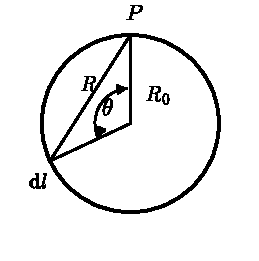
\includegraphics[width=5cm]{fig3.pdf}\\[0.3em]
{\small 图 3}
\end{minipage}\par\nopagebreak

但是，这个积分在积分下限呈对数发散，必须在$\theta\sim a/R_{0}$的数值处截断，该值对应于$P$点到线元$\mathrm{d}\bm{l}$的原子距离（$\sim a$）. 积分以对数精确度定义在区域$a/R_{0}\ll\theta\ll\pi$内，并等于
\begin{equation*}
\int_{\sim a/R_{0}}^{\sim 1}\frac{2\,\mathrm{d}\theta}{\theta}=2\ln\frac{R_{0}}{a},
\end{equation*}
因此
\begin{equation}
v=\frac{\kappa}{2R_{0}}\ln\frac{R_{0}}{a}
=\frac{\hbar}{2mR_{0}}\ln\frac{R_{0}}{a}.
\label{29x1}
\end{equation}
以同样的对数精确度，涡环的能量为：
\begin{equation}
\varepsilon=2\pi^{2}R_{0}\rho_{s}\frac{\hbar^{2}}{m^{2}}\ln\frac{R_{0}}{a}
\label{29x2}
\end{equation}
［在公式\eqref{29.8}中，将$R$换成$R_{0}$，将$L$换为$2\pi R_{0}$］. 能量$\varepsilon$与速度$v$是以关系式$\mathrm{d}\varepsilon/\mathrm{d}p=v$联系起来的，式中$p$是环的动量. 由此
\begin{equation*}
\mathrm{d}p=\frac{\mathrm{d}\varepsilon}{v}
=4\pi^{2}\rho_{s}\frac{\hbar}{m}R_{0}\,\mathrm{d}R_{0}
\end{equation*}
（若保持对数精确度，则求微分时应把大的对数看作是常数），所以
\begin{equation}
p=2\pi^{2}\rho_{s}\frac{\hbar}{m}R_{0}^{2}
\label{29x3}
\end{equation}
公式\eqref{29x2}，\eqref{29x3}以参数形式（参数为$R_{0}$）确定了涡环能量$\varepsilon(p)$的依赖关系.

应注意，由于得出公式\eqref{29x1}的积分具有对数特征，这个公式（其中的记号作了一定的变更）对于任何形状弯曲涡线的每条给定线元的移动速度$v$仍旧成立：
\begin{equation}
\bm{v}=\frac{\kappa}{2R_{0}}\bm{b}\ln\frac{\lambda}{a}
\label{29x4}
\end{equation}
这里$\bm{b}$为垂直于涡线在给定点的切平面的单位矢量（副法线矢量）；$R_{0}$是涡线在该点的曲率半径；$\lambda$为涡线曲率发生变化的特征距离.

2. 试求直线形涡线微振动的色散律（W.\,Thomson, 1880）.

{\heiti 解：}我们选取涡线作为$z$轴，并令矢量$\bm{r}=(x,y)$表示涡线振动时线上各点的位移；它是$z$和时间$t$的函数，其形式为$\exp[\mathrm{i}(kz-\omega t)]$. 涡线各点的速度可由公式\eqref{29x4}得出，在该情况下应把此公式中的$\lambda$理解为振动的波长（$\lambda\sim1/k$）：
\begin{equation*}
\bm{v}=\frac{\mathrm{d}\bm{r}}{\mathrm{d}t}=-\mathrm{i}\omega\bm{r}
=\frac{\kappa}{2}\ln\frac{1}{ak}\,\frac{\bm{b}}{R_{0}},
\end{equation*}
副法线矢量$\bm{b}=\bm{t}\times\bm{n}$，这里$\bm{t}$和$\bm{n}$分别为曲线的切线和主法线的单位矢量. 根据熟知的微分几何公式，$\mathrm{d}^{2}\bm{r}/\mathrm{d}l^{2}=\bm{n}/R_{0}$，此处$l$为沿曲线计得的长度. 当微振动时，涡线只呈微小的弯曲，因此可以取$l\approx z$及$\bm{t}=\bm{n}_{z}$（沿$z$轴的单位矢量）；于是
\begin{equation*}
\frac{\bm{b}}{R_{0}}\approx\bm{n}_{z}\times\frac{\mathrm{d}^{2}\bm{r}}{\mathrm{d}z^{2}}
=-k^{2}\bm{n}_{z}\times\bm{r}.
\end{equation*}
因此，我们求得涡线的运动方程：
\begin{equation*}
-\mathrm{i}\omega\bm{r}
=-\frac{\kappa k^{2}}{2}\bm{n}_{z}\times\bm{r}\ln\frac{1}{ak}.
\end{equation*}
若表成展开式，上式可给出关于$x$和$y$的两个线性齐次方程的方程组；使这个方程组的行列式等于零，便得到所求的$\omega$和$k$之间的关系：
\begin{equation*}
\omega=\frac{\kappa k^{2}}{2}\ln\frac{1}{ak}.
\end{equation*}

\end{xiti}

\section{非均匀玻色气体}

在§25我们研究了粒子间有弱排斥的近理想玻色气体的性质. 然而，如气体是空间非均匀的，这个系统就会出现新的重要量子特性. 本节我们将把理论推广到非均匀气体情况.

现在研究温度为绝对零度时的弱非理想气体. 在此气体中，几乎它的全部粒子都处于凝聚态. 用$\Psi$算符来表述，是指算符“非凝聚体”部分（$\hat{\Psi}'$）小于它的平均值，即小于凝聚体波函数$\Xi$. 算符$\hat{\Psi}(t,\bm{r})$满足“薛定谔方程”(7.8). 如只考虑无自旋粒子的成对相互作用，此方程的形式如下（略去$U^{(1)}$的上标(1).）
\begin{equation}
\begin{aligned}
\mathrm{i}\hbar\frac{\partial}{\partial t}\hat{\Psi}(t,\bm{r})
&=\left(-\frac{\hbar^{2}}{2m}\Delta+\mu+U(\bm{r})\right)\hat{\Psi}(t,\bm{r})+{}\\
&+\int\hat{\Psi}^{+}(t,\bm{r}')U^{(2)}(\bm{r}-\bm{r}')\hat{\Psi}(t,\bm{r}')\,\mathrm{d}^{3}x'\,\hat{\Psi}(t,\bm{r}).
\end{aligned}
\label{30.1}
\end{equation}

然而，在\eqref{30.1}式中简单地将$\Psi(t,\bm{r})$换成$\Xi(t,\bm{r})$，在一般情形是不正确的. 因为，这个代换并未考虑在粒子成对势作用半径量级的距离上有强烈的相互作用. 这个困难是可以回避的. 如§6和§25所为，形式上将真实相互作用势换成与散射长度$a$值相同并允许使用微扰论的势. 此时，在\eqref{30.1}式中将$\hat{\Psi}$换成$\Xi$在所有距离上都是允许的. 这里认为函数$\Xi(t,\bm{r})$在原子距离内变化很小. 我们可以将代换后的$\Xi(t,\bm{r})$从积分号下提出来，于是该积分归结为$\int U^{(2)}(\bm{r})\,\mathrm{d}^{3}x\equiv U_{0}$. 这样，得出形如下面的$\Xi(t,\bm{r})$的待求方程
\begin{equation}
\mathrm{i}\hbar\frac{\partial}{\partial t}\Xi(t,\bm{r})
=\left(-\frac{\hbar^{2}}{2m}\Delta-\mu+U(\bm{r})\right)\Xi(t,\bm{r})
+U_{0}|\Xi(t,\bm{r})|^{2}\Xi(t,\bm{r}).
\label{30.2}
\end{equation}
如在§25，现在我们应该认为描述原子间相互作用的常数$U_{0}$用精确的散射长度公式(6.2)表示成：
\begin{equation}
U_{0}=\frac{4\pi\hbar^{2}}{m}a.
\label{30.3}
\end{equation}

应强调指出，凝聚体波函数$\Xi(t,\bm{r})$，正如§27指出的，是经典宏观量，这时它所满足的方程\eqref{30.2}却显含普朗克常量$\hbar$.

在定态，函数$\Xi$与时间无关（我们提醒，方程\eqref{30.1}已对应哈密顿量$\hat{H}'=\hat{H}-\hat{N}\mu$）因此，这样的状态用下列方程\footnote{E.\,P.\,Gross(1961)和Л.\,П.\,Питаевский(1961)在讨论下面的玻色气体中的涡线问题时得出方程(30.2)和(30.4). 类似(30.4)的方程，早先被В.\,Л.\,Гинзбург和Л.\,П.\,Питаевский(1958)在$\lambda$点附近液氦超流理论中研究过. 在此二问题里系数的意义完全不同. 然而，此二方程形式上的相似性允许将对氦中涡线的解用于玻色气体. 这个解如图4所示.}描述：
\begin{equation}
\left(-\frac{\hbar^{2}}{2m}\Delta-\mu+U(\bm{r})\right)\Xi(\bm{r})
+U_{0}|\Xi(\bm{r})|^{2}\Xi(\bm{r})=0.
\label{30.4}
\end{equation}

应指出，在无外场时从方程\eqref{30.4}得出均匀气体化学势等于$\mu=nU_{0}$（$n$为气体密度）. 这对应于博戈留波夫理论的第一级近似(25.6).

所得方程的重要应用是近理想玻色气体涡线的结构问题. 正如指出过，液体中的涡线本身的粗细以原子距离来衡量. 然而在近理想玻色气体，情况就是另外的样子了. 这里，涡线“芯”所在介质的性质有显著变化. 在下边我们将看到，芯具有宏观粗细，它的结构可以用上边得到的方程来描述. 假如不存在外场，$n$是无穷远处非微扰的气体密度. 设\eqref{30.3}式中$\mu=nU_{0}$，得出方程
\begin{equation}
-\frac{\hbar^{2}}{2m}\Delta\Xi(\bm{r})
+U_{0}\{|\Xi(\bm{r})|^{2}-n\}\Xi(\bm{r})=0.
\label{30.5}
\end{equation}

\par\nopagebreak\noindent\begin{minipage}{\linewidth}\centering
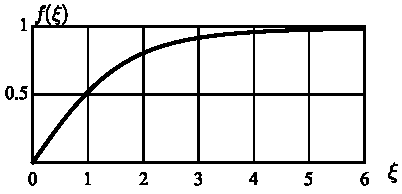
\includegraphics[width=7.5cm]{fig4.pdf}\\[0.3em]
{\small 图 4}
\end{minipage}\par\nopagebreak

直线涡线对应如下形的解
\begin{equation}
\Xi=\sqrt{n}\,\mathrm{e}^{\mathrm{i}\varphi}f\left(\frac{r}{r_{0}}\right),\quad
r_{0}=\frac{\hbar}{\sqrt{2mU_{0}n}}
\label{30.6}
\end{equation}
式中$r$和$\varphi$分别是到涡轴距离和绕轴极角. 此函数的相位对应于环流值\eqref{29.7}. 平方$|\Xi|^{2}$是凝聚体中粒子数密度. 在所讨论的近似下，此数密度与气体总密度$|\Xi|^{2}$一致. 当$r\to\infty$，气体总密度应趋于给定的数值$n$，而函数$f$相应地趋于1.

引入一个量纲为1的变量$\xi=r/r_{0}$，得出函数$f(\xi)$的方程
\begin{equation}
\frac{1}{\xi}\frac{\mathrm{d}}{\mathrm{d}\xi}\left(\xi\frac{\mathrm{d}f}{\mathrm{d}\xi}\right)
-\frac{f}{\xi^{2}}+f-f^{3}=0.
\label{30.7}
\end{equation}

图4表示由方程\eqref{30.7}用数值积分得出的解. 当$\xi\to0$时方程的解与$\xi$成正比地趋于零. 当$\xi\to\infty$时，解按$f=1-\dfrac{1}{2\xi^{2}}$的规律趋于1.

参数$r_{0}$决定涡“芯”半径的数量级. 现在引入散射长度以代替$U_{0}$，按照(6.2)式中$U_{0}=4\pi\hbar^{2}a/m$，求得：
\begin{equation*}
r_{0}\sim n^{-1/3}\eta^{-1/2}\gg n^{-1/3},
\end{equation*}
式中$\eta=an^{1/3}$为气体参数. 如果气体参数足够小，则这个半径实际上大于原子间距.

气体非均匀性起显著作用的另一个问题是气体在外场内的问题. 设气体处在势能$U(\bm{r})<0$的引力场内（与此对应的实际实验情形是原子阻留于“磁阱”内）. 基态波函数可以选为实的并满足方程\eqref{30.4}. 在无穷远处函数应趋于零，而化学势$\mu$从归一化条件来确定：
\begin{equation}
\int(\Xi(\bm{r}))^{2}\,\mathrm{d}^{3}x=N,
\label{30.8}
\end{equation}
式中$N$为气体粒子总数. 在一般情况，方程\eqref{30.4}只能数值解. 然而存在两种极限情况，问题可以大大化简.

因为方程\eqref{30.4}中不同项的相对重要性决定于\eqref{30.6}式所定义的量$r_{0}$与气体“云”特征线度$R$之比. 简单的估算表明，含相互作用项$U_{0}$与含拉普拉斯算子$\Delta$项之比的数量级为$(R/r_{0})^{2}$.

于是，当$R\ll r_{0}$时相互作用完全不重要. 此时方程\eqref{30.4}就归于粒子在势$U(\bm{r})$内的薛定谔方程. 这表明气体可以算作理想的，而且所有的原子都要凝聚，此状态对应于场$U(\bm{r})$内的每个原子都处在基态.

相反的极限情况是：方程可以略去拉普拉斯算子$\Delta$，则气体密度简单地由下式给出
\begin{equation}
(\Xi(\bm{r}))^{2}=n(\bm{r})=\frac{1}{U_{0}}(\mu-U(\bm{r}))
\label{30.9}
\end{equation}
此式表述化学势在外场内不变的经典条件. 我们注意到在这种近似下，气体有由方程$\mu-U(\bm{r})=0$所决定的清楚的界限. 化学势在区域$U(\bm{r})<\mu$上通过积分\eqref{30.9}式而求得

\begin{xiti}

试求近理想玻色气体中的元激发谱，这里将元激发谱看作是凝聚体波函数微振动的色散律.

{\heiti 解：}现在来研究$\Xi$在恒定平均值$\sqrt{n}$附近的微振动：
\begin{equation*}
\Xi=\sqrt{n}+A\mathrm{e}^{\mathrm{i}(\bm{k}\cdot\bm{r}-\omega t)}
+B^{*}\mathrm{e}^{-\mathrm{i}(\bm{k}\cdot\bm{r}-\omega t)},
\end{equation*}
这里$A$，$B^{*}$是复数微振幅. 把这个表达式代入方程\eqref{30.2}，其中外势$U$取为零. 使\eqref{30.2}式线性化并将带有不同指数因子的各项分开，则得方程组：
\begin{equation*}
\left\{\begin{array}{l l}
\hbar\omega A=\dfrac{p^{2}}{2m}A+nU_{0}(A+B),\\[0.8em]
-\hbar\omega B=\dfrac{p^{2}}{2m}B+nU_{0}(A+B),
\end{array}\right.
\end{equation*}
其中$\bm{p}=\hbar\bm{k}$. 由此令方程组的行列式等于零，求得：
\begin{equation*}
(\hbar\omega)^{2}=\left(\frac{p^{2}}{2m}\right)^{2}+\frac{p^{2}}{m}nU_{0}.
\end{equation*}
此式与(25.10)式相同.

\end{xiti}

\section[玻色液体的格林函数]{玻色液体的格林函数\footnote{在§31—§33，§35中用的是$\hbar=1$的单位制.}}

玻色液体格林函数这一数学工具的建立，在许多地方跟费米液体的同类工具类似. 这里不再重复全部讨论，但我们首先引入一些基本定义和公式，并且着重指出它们的区别. 这些区别既与不同的统计法有关，也与凝聚体的存在有关\footnote{将格林函数这一数学方法运用于具有凝聚体的玻色体系统，属于С.\,Т.\,Беляев(1958)的工作.}. 与本章上述几节一样，现在也假定液体粒子是无自旋的.

在定义玻色液体格林函数时，应当把算符表成(26.4)式，并将\textbf{凝聚体}部分从海森伯$\psi$算符中分离出去. 格林函数用非凝聚体部分算符并根据
\begin{equation}
G(X_{1},X_{2})=-\mathrm{i}\langle T\hat{\Psi}'(X_{1})\hat{\Psi}'^{+}(X_{2})\rangle
\label{31.1}
\end{equation}
定义，这里还用括号$\langle\cdots\rangle$表示对系统的基态求平均，$T$是编时乘积记号. 但这与费米子的情况不同，现在置换各$\psi$算符以使它们排在需要的位置时并不需改变乘积的符号，因此有与(7.10)式不同的形式：
\begin{equation}
\mathrm{i}G(X_{1},X_{2})=
\left\{\begin{array}{l l}
\langle\hat{\Psi}'(X_{1})\hat{\Psi}'^{+}(X_{2})\rangle, & t_{1}>t_{2};\\[0.3em]
\langle\hat{\Psi}'^{+}(X_{2})\hat{\Psi}'(X_{1})\rangle, & t_{1}<t_{2}.
\end{array}\right.
\label{31.2}
\end{equation}

平均值同\eqref{31.1}式是一样的，但应以全$\psi$算符代替非凝聚体部分算符，于是应得出：
\begin{equation}
-\mathrm{i}\langle T\hat{\Psi}(X_{1})\hat{\Psi}^{+}(X_{2})\rangle
=-\mathrm{i}n_{0}+G(X_{1},X_{2}),
\label{31.3}
\end{equation}
式中$n_{0}$为凝聚体中粒子数密度\footnote{像对待费米系统一样，我们将研究在给定化学势$\mu$值(而不是给定$N$)的情况下玻色系统的状态. 相应地，(7.1)式的$\hat{H}'=\hat{H}-\mu\hat{N}$这个差起着系统的哈密顿量的作用. 这时$\psi$算符的凝聚体部分与时间无关.}. 在均匀液体中，函数$G$当然只与差值$X=X_{1}-X_{2}$有关.

非凝聚体密度矩阵$\rho'$，可通过格林函数按照下式表达出来：
\begin{equation}
N\rho'(\bm{r}_{1},\bm{r}_{2})
=\mathrm{i}G(t,\bm{r}_{1};t_{1}+0,\bm{r}_{2})
=\mathrm{i}G(t=-0,\bm{r})
\label{31.4}
\end{equation}
［注意，与(7.18)式的总符号不同］. 其中当$\bm{r}_{1}=\bm{r}_{2}$时，可得到非凝聚体粒子数总密度：
\begin{equation}
\frac{N}{V}-n_{0}=\mathrm{i}G(t=-0,\bm{r}=0)
\label{31.5}
\end{equation}
［比较(7.19)式］.

现在还按照公式(7.21—7.22)变到动量表象中去. 函数$G(\omega,\bm{p})$的归一化可用下列公式表出：
\begin{equation}
\frac{N}{V}=n_{0}+\mathrm{i}\lim_{t\to-0}\int G(\omega,\bm{p})\,\mathrm{e}^{-\mathrm{i}\omega t}\frac{\mathrm{d}\omega\,\mathrm{d}^{3}p}{(2\pi)^{4}}
\label{31.6}
\end{equation}
［比较(7.24)式］.

对于动量表象中的玻色系统格林函数，可以得到和§8中对于费米系统同样的展开式. 经完全类似的计算，首先得出公式：
\begin{equation}
\begin{aligned}
G(\omega,\bm{p})=(2\pi)^{3}\sum_{m}\Big\{
&\frac{A_{m}\delta(\bm{p}-\bm{p}_{m})}{\omega+E_{0}(N)-E_{m}(N+1)+\mu+\mathrm{i}0}-{}\\
&-\frac{B_{m}\delta(\bm{p}-\bm{p}_{m})}{\omega-E_{0}(N)+E_{m}(N-1)+\mu-\mathrm{i}0}\Big\},
\end{aligned}
\label{31.7}
\end{equation}
其中
\begin{equation*}
A_{m}=|\langle0|\hat{\psi}'(0)|m\rangle|^{2},\quad
B_{m}=|\langle m|\hat{\psi}'(0)|0\rangle|^{2}
\end{equation*}
［$\hat{\psi}'(\bm{r})$为非凝聚体的薛定谔算符］\footnote{公式(31.7)对应于公式(8.7). 因为粒子无自旋，所以现在没有1/2这一因子. 注意，(31.7)式第二项前的符号与(8.7)式不同.}. 为了导出这个展开式的最终形式，我们指出：在粒子数$N$不变的情况下，玻色系统的激发态能量和基态能量的恒为正的差值便定义为该系统中的激发能量$\varepsilon_{m}(N)$. 考虑到$E_{0}(N)+\mu\approx E_{0}(N+1)$，因此求得：
\begin{equation*}
\begin{aligned}
&E_{m}(N+1)-E_{0}(N)-\mu\approx E_{m}(N+1)-E_{0}(N+1)=\varepsilon_{m}(N+1)>0,\\
&E_{m}(N-1)-E_{0}(N)+\mu\approx E_{m}(N-1)-E_{0}(N-1)=\varepsilon_{m}(N-1)>0.
\end{aligned}
\end{equation*}
但是添入或取出一个粒子，只在相对数量级$\sim\dfrac{1}{N}$的各项上系统的性质才发生变化. 对于宏观系统来说，这些项小得可以忽略，因此应当认为激发能$\varepsilon_{m}(N\pm1)$和$\varepsilon_{m}(N)$是相等的. 所以，最终求得：
\begin{equation}
G(\omega,p)=(2\pi)^{3}\sum_{m}\Big\{
\frac{A_{m}\delta(\bm{p}-\bm{p}_{m})}{\omega-\varepsilon_{m}+\mathrm{i}0}
-\frac{B_{m}\delta(\bm{p}-\bm{p}_{m})}{\omega+\varepsilon_{m}-\mathrm{i}0}\Big\}.
\label{31.8}
\end{equation}
从而用获得(8.14)式的同样方法不难求出：对于玻色系统，格林函数的虚部永远是负的：
\begin{equation}
\mathrm{Im}\ G(\omega,p)<0.
\label{31.9}
\end{equation}
格林函数当$\omega\to\infty$时的渐近形式仍旧和费米系统的情况一样：
\begin{equation}
G(\omega,\bm{p})\to1/\omega,\quad\text{当}\ |\omega|\to\infty\ \text{时}
\label{31.10}
\end{equation}
［比较(8.15)式］. 在推导这个结果时应考虑如下对易规则：
\begin{equation*}
\hat{\psi}(t,\bm{r}_{1})\hat{\psi}^{+}(t,\bm{r}_{2})
-\hat{\psi}^{+}(t,\bm{r}_{2})\hat{\psi}(t,\bm{r}_{1})
=\delta(\bm{r}_{1}-\bm{r}_{2}).
\end{equation*}
此式现在是以算符$\hat{\psi}$和$\hat{\psi}^{+}$的对易子代替反对易子\footnote{在函数$G$的定义中分离出去$\psi$算符的凝聚体部分在这里是无关紧要的，因为$\delta$函数$\delta(\omega)\delta(\bm{p})$在动量表象中对应于(31.3)式中的常数项$-\mathrm{i}n_{0}$，它并不影响(31.10)式.}.

其次，进行如§8中所作的讨论，可得到一个主要结果，即格林函数的各极点确定元激发谱：
\begin{equation}
G^{-1}(\varepsilon,p)=0,
\label{31.11}
\end{equation}
而且只应取这个方程的正根；和(8.16)式不同的是，这里不需要从$\varepsilon$中减去$\mu$.

格林函数在自身的极点附近具有下列形式：
\begin{equation}
G(\omega,p)\approx\frac{Z_{+}}{\omega\mp\varepsilon(p)},\quad
Z_{+}>0,\ Z_{-}<0.
\label{31.12}
\end{equation}
极点留数的符号与$\omega$的符号一致，这一点是根据\eqref{31.8}式中系数$A_{m}$，$B_{m}$的正定性得出的［但留数的大小不受任何类似于费米系统(10.4)式那样条件的限制］. 和§8中的做法一样，利用表达式\eqref{31.12}不难证明：不等式\eqref{31.9}自然保证准粒子衰减系数的正定性，也就是说，当$\varepsilon$值向复数区域移动时，需要的符号是$-\mathrm{Im}\ \varepsilon>0$.

非凝聚体粒子可能转为凝聚体以及进行相反的过程，除函数\eqref{31.1}之外，还将使玻色系统格林函数这一数学工具中自然也出现如下函数（我们在§33中将会看到）：
\begin{equation}
\mathrm{i}F(X_{1},X_{2})
=\langle N-2|T\hat{\Psi}'(X_{1})\hat{\Psi}'(X_{2})|N\rangle,
\label{31.13}
\end{equation}
\begin{equation}
\begin{aligned}
\mathrm{i}F^{+}(X_{1},X_{2})
&=\langle N|T\hat{\Psi}'^{+}(X_{1})\hat{\Psi}'^{+}(X_{2})|N-2\rangle={}\\
&=\langle N+2|T\hat{\Psi}'^{+}(X_{1})\hat{\Psi}'^{+}(X_{2})|N\rangle.
\end{aligned}
\label{31.14}
\end{equation}
其中跃迁矩阵元是对于系统中总粒子数的变化的，记号$|N\rangle$表征$N$个粒子的系统的基态（\eqref{31.14}式中最后一个等式在精确到数值$\sim1/N$的情况下是成立的，对比95页上的脚注）. 这样定义的函数$F$和$F^{+}$，称作\textbf{反常格林函数}. 现在我们来证明：在均匀并静止的液体中，函数$F$和$F^{+}$彼此相等.

同函数$G$一样，均匀液体的函数$F$和$F^{+}$只与差值$X=X_{1}-X_{2}$有关\footnote{函数$F$与时间之和$t_{1}+t_{2}$无关，这一性质与哈密顿量的定义式$\hat{H}'=\hat{H}-\mu\hat{N}$中含有$-\mu\hat{N}$这一项有关. 因而由不同粒子数系统能量本征值之差可消去这一项：
\begin{equation*}
E(N+2)-E(N)\approx 2\,\partial E/\partial N=2\mu
\end{equation*}
相应地从算符$\hat{\Psi}'_{1}\hat{\Psi}'_{2}$的矩阵元中消去因子$\exp[-\mathrm{i}\mu(t_{1}+t_{2})]$.}. 此时，由于置换$X_{1}$和$X_{2}$只能改变乘积中算符的排列顺序，而排列顺序总会由编时手续建立. 所以
\begin{equation}
F(X)=F(-X).
\label{31.15}
\end{equation}
当然，由此得出：在动量表象中$F$也是本身宗量的偶函数：
\begin{equation}
F(P)=F(-P).
\label{31.16}
\end{equation}
其次，$F$和$F^{+}$之间确定的关系，是由静止液体海森伯$\psi$算符的下述性质得出的结果\footnote{这个问题，可用下述方法证明. 算符$\hat{a}_{\bm{p}}$，$\hat{a}^{+}_{\bm{p}}$的一切不等于零的矩阵元都能定义为实量［见第三卷(64.7—8)］；就此意义来说，这两个算符都是实的，即$\hat{a}^{+}_{\bm{p}}\equiv\tilde{\hat{a}}^{+}_{\bm{p}}=\tilde{\hat{a}}_{\bm{p}}$. 因此薛定谔$\psi$算符
\begin{equation*}
\hat{\psi}(\bm{r})=V^{-1/2}\sum_{\bm{p}}\hat{a}_{\bm{p}}\,\mathrm{e}^{\mathrm{i}\bm{p}\cdot\bm{r}},
\end{equation*}
具有$\hat{\psi}^{+}(\bm{r})=\tilde{\hat{\psi}}(-\bm{r})$这一性质. 由此也可得出海森伯算符
\begin{equation*}
\hat{\Psi}(t,\bm{r})=\exp(\mathrm{i}\hat{H}t)\hat{\psi}(\bm{r})\exp(-\mathrm{i}\hat{H}t)
\end{equation*}
的等式(31.17)，这是容易证明的，只要注意下列事实即可：对于无自旋相互作用系统，哈密顿量$\hat{H}$是实的（因此$\hat{H}^{+}=\hat{H}$），由于系统是各向同性的，所以$\hat{H}(-\bm{r})=\hat{H}(\bm{r})$. 但是，需要强调一下：哈密顿量具有实数性，其意思是指，在液体中不存在宏观超流运动. 对于玻色凝聚系统，哈密顿量依赖于宏观参量——凝聚体波函数$\Xi$. 在运动液体中，这个参量是复的，随之哈密顿量也是复的（但自然都是厄米的）.}：
\begin{equation}
\hat{\Psi}^{+}(t,\bm{r})=\tilde{\Psi}(-t,-\bm{r}).
\label{31.17}
\end{equation}
譬如说，令$t_{2}>t_{1}$，而有：
\begin{equation*}
\begin{aligned}
&\mathrm{i}F^{+}(X_{1},X_{2})
=\langle N+2|\tilde{\Psi}'^{+}(X_{2})\tilde{\Psi}'^{+}(X_{1})|N\rangle={}\\
&=\langle N|\tilde{\Psi}'^{+}(X_{1})\tilde{\Psi}'^{+}(X_{2})|N+2\rangle={}\\
&=\langle N|\hat{\Psi}'(-X_{1})\hat{\Psi}'(-X_{2})|N+2\rangle={}\\
&=\mathrm{i}F(-X_{1},-X_{2}).
\end{aligned}
\end{equation*}
或$F^{+}(X)=F(-X)$. 考虑\eqref{31.15}式，从而得出所求的等式：
\begin{equation}
F^{*}(X)=F(X).
\label{31.18}
\end{equation}

将函数$F(X)$通过$\psi$算符的矩阵元表达出来后，便可以得到类似于\eqref{31.8}式的$F(\omega,\bm{p})$的展开式，因而也可以阐明该函数的极点问题；但在这里我们不研究这个问题. 仅指出：函数$F(\omega,\bm{p})$的极点与函数$G(\omega,\bm{p})$的极点相同.

在本节的最后，我们将算出理想玻色气体的格林函数$G^{(0)}$. 首先应当指出：因为在这种气体的基态，所有粒子都处凝聚体中，所以非凝聚体粒子的湮没算符$\hat{\psi}'$作用到基态波函数上，将使该波函数变成零. 因此函数$G^{(0)}(t,\bm{r})$只有当$t=t_{1}-t_{2}>0$时才不为零. ［根据\eqref{31.2}式，如果产生算符$\hat{\Psi}'^{+}$首先作用的话］.

虽然对于理想气体来说化学势$\mu=0$，但在这里把化学势$\mu$视作预先未确定的自由参量时，我们不能使$\mu=0$；这一点，对于在图技术中进一步将函数$G^{(0)}$应用于任意液体时是很必要的，在这样的液体中$\mu$恰好起这种参量作用，与此相应，算符$\hat{\Psi}'_{0}(t,\bm{r})$可写成
\begin{equation}
\hat{\Psi}'_{0}(t,\bm{r})=\frac{1}{\sqrt{V}}\sum_{\bm{p}\neq0}\hat{a}_{\bm{p}}
\exp\left[\mathrm{i}\left(\bm{p}\cdot\bm{r}-\frac{p^{2}}{2m}t+\mu t\right)\right]
\label{31.19}
\end{equation}
［与(26.1)式只差指数函数因子$\mathrm{e}^{\mathrm{i}\mu t}$］. 按照\eqref{31.2}式，将此表达式代入$G^{(0)}$的定义式时应注意：当取平均时（即取对角矩阵元），只有乘积$\hat{a}_{\bm{p}}\hat{a}^{+}_{\bm{p}}$和$\hat{a}^{+}_{\bm{p}}\hat{a}_{\bm{p}}$能够给出不等于零的结果；但因为在气体的基态时$\bm{p}\neq0$的粒子的一切状态的占有数都等于零，所以
\begin{equation*}
\langle\hat{a}^{+}_{\bm{p}}\hat{a}_{\bm{p}}\rangle=0,\quad
\langle\hat{a}_{\bm{p}}\hat{a}^{+}_{\bm{p}}\rangle=1.
\end{equation*}
然后以通常的方法由对$\bm{p}$求和过渡为求积分，则得：
\begin{equation}
G^{(0)}(t,\bm{r})=\left\{\begin{array}{l}
-\mathrm{i}\int\exp\Big(-\mathrm{i}\dfrac{p^{2}}{2m}t+\mathrm{i}\mu t+\mathrm{i}\bm{p}\cdot\bm{r}\Big)\dfrac{\mathrm{d}^{3}p}{(2\pi)^{3}},
\ \text{当}\ t>0\ \text{时};\\[1.2em]
0,\ \text{当}\ t<0\ \text{时};
\end{array}\right.
\label{31.20}
\end{equation}
从而对于动量表象中的格林函数，有：
\begin{equation*}
G^{(0)}(\omega,\bm{p})
=-\mathrm{i}\int_{0}^{\infty}\exp\Big(-\mathrm{i}\frac{p^{2}}{2m}t+\mathrm{i}\mu t+\mathrm{i}\omega t\Big)\mathrm{d}t.
\end{equation*}
积分时应借助于公式
\begin{equation}
\int_{0}^{\infty}\mathrm{e}^{\mathrm{i}\alpha t}\,\mathrm{d}t=\frac{\mathrm{i}}{\alpha+\mathrm{i}0}
\label{31.21}
\end{equation}
（在被积式中引入因子$\mathrm{e}^{-\lambda t}$，其中$\lambda>0$，此后取$\lambda\to0$的极限）. 最终
\begin{equation}
G^{(0)}(\omega,\bm{p})=\left(\omega-\frac{p^{2}}{2m}+\mu+\mathrm{i}0\right)^{-1}.
\label{31.22}
\end{equation}

至于函数$F$，则对于理想气体来说$F^{(0)}(X)=0$，根据定义\eqref{31.13}式这是显而易见的，在\eqref{31.13}式中两个算符湮没了非凝聚体的粒子. 因此在动量表象中也有
\begin{equation}
F^{(0)}(\omega,\bm{p})=0.
\label{31.23}
\end{equation}
此等式表明这一事实：当$T=0$时，只是由于相互作用才出现非凝聚体粒子.

\begin{xiti}

试求声子场的格林函数，该函数定义为
\begin{equation}
D(X_{1},X_{2})\equiv D(X_{1}-X_{2})
=-\mathrm{i}\langle T\hat{\rho}'(X_{1})\hat{\rho}'(X_{2})\rangle,
\label{31x1}
\end{equation}
式中角括号表征按场的基态求平均；$\hat{\rho}'$为(24.10)式中的密度算符，编时乘积可按\eqref{31.2}式的规则展开.

{\heiti 解：}把(24.10)式代入定义\eqref{31x1}时应注意：因为在基态上声子状态的所有占有数都等于零，所以只有平均值$\langle\hat{C}^{+}_{\bm{k}}\hat{C}_{\bm{k}}\rangle=1$不等于零. 然后由对$\bm{k}$求和变为求积分，得：
\begin{equation*}
D(t,\bm{r})=\int\frac{\rho k}{2\mathrm{i}u}\,
\mathrm{e}^{\mathrm{i}(\bm{k}\cdot\bm{r}\mp ukt)}\,\frac{\mathrm{d}^{3}k}{(2\pi)^{3}},
\end{equation*}
这里指数中的“$-$”和“$+$”两个符号分别对应于$t>0$和$t<0$的情况（积分中对于$t<0$的情况，积分变量进行了变换：$\bm{k}\to-\bm{k}$）. 被积式（无因子$\mathrm{e}^{\mathrm{i}\bm{k}\cdot\bm{r}}$时）就是函数$D(t,\bm{r})$按坐标的傅里叶展开的分量. 同时也按时间将函数分解，便得到动量表象中的格林函数：
\begin{equation*}
D(\omega,\bm{k})=\frac{\rho k}{2\mathrm{i}u}
\bigg\{\int_{0}^{\infty}\mathrm{e}^{\mathrm{i}(\omega-uk)t}\,\mathrm{d}t
+\int_{-\infty}^{0}\mathrm{e}^{\mathrm{i}(\omega+uk)t}\,\mathrm{d}t\bigg\},
\end{equation*}
借助公式\eqref{31.21}求出积分，则得：
\begin{equation*}
D(\omega,\bm{k})=\frac{\rho k}{2u}\left[
\frac{1}{\omega-uk+\mathrm{i}0}-\frac{1}{\omega+uk-\mathrm{i}0}\right]
=\frac{\rho k^{2}}{\omega^{2}-u^{2}k^{2}+\mathrm{i}0}.
\end{equation*}

\end{xiti}

\section{玻色液体的图技术}

下面建立用于计算玻色系统格林函数的图技术，这和在§12—§13中对于费米系统的作法是一样的. 同以前一样，我们来定出图技术规则. 这个系统分子间的成对相互作用以如下算符描述：
\begin{equation}
\hat{V}(t)=\frac{1}{2}\int\hat{\Psi}^{+}(t,\bm{r}_{1})\hat{\Psi}^{+}(t,\bm{r}_{2})
U(\bm{r}_{1}-\bm{r}_{2})\hat{\Psi}(t,\bm{r}_{2})\hat{\Psi}(t,\bm{r}_{1})\,
\mathrm{d}^{3}x_{1}\,\mathrm{d}^{3}x_{2}.
\label{32.1}
\end{equation}

具有凝聚体的玻色液体的特点，首先在于全部海森伯$\psi$算符都应当表为$\hat{\Psi}=\hat{\Psi}'+\Xi$的形式，其中$\hat{\Psi}'$为非凝聚体部分，$\Xi$是凝聚体波函数，对于静止液体来说，$\Xi$只是一个实数$\sqrt{n_{0}}$\footnote{应当强调：因为这个量是从精确的海森伯$\psi$算符分离出来的，所以$n_{0}$是$T=0$时液体中凝聚体密度的精确值.}. 作这样的代换之后，算符\eqref{32.1}可以分解为由四个到零个算符$\hat{\Psi}'$（连同相应因子$\sqrt{n_{0}}$的附加数）的各项所构成的级数.

在§12中关于变到相互作用绘景的所有叙述仍然完全有效，而借助维克定理（与以前不同的，只是现在在求平均的乘积中置换$\psi$算符不需要变号）可以将得到的表达式实行进一步展开. 但是算符\eqref{32.1}分解成各种不同项，它们将导致在费曼图中出现新的图元素. 我们可以立刻写出最终的动量表象中的这些图元素.

在图的每个顶点上，同以前一样汇聚了三条线：一条虚线［相当于具有4-动量$Q=(q_{0},\bm{q})$的因子$-\mathrm{i}U(Q)$］和两条粒子线——一条入射线及一条出射线. 但这时应当将凝聚体粒子和非凝聚体粒子区别开来. 各实线现在对应于非凝聚体粒子，这种线［具有4-动量$P=(\omega,\bm{p})$］同以前一样对应于因子$\mathrm{i}G^{(0)}(P)$. 凝聚体粒子线则以波纹线来表示；用这些线来描述4-动量$P=0$，它们相应于因子$\sqrt{n_{0}}$\footnote{更准确地说，入射到顶点的波纹线相应于因子$\Xi$，而出射线相应于因子$\Xi^{*}$，由于$\Xi$是个实数，所以这两个因子实际上是相同的.}. 因此，出现了四种形式的顶点：
\begin{equation}
\begin{tabular}{c@{\hspace{2.5em}}c@{\hspace{2.5em}}c@{\hspace{2.5em}}c}
\raisebox{-0.3\height}{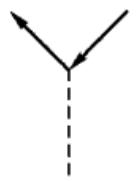
\includegraphics[height=1.55cm]{feyn32-2a.png}} &
\raisebox{-0.3\height}{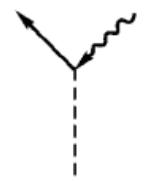
\includegraphics[height=1.55cm]{feyn32-2b.png}} &
\raisebox{-0.3\height}{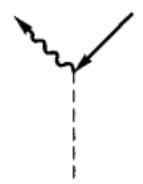
\includegraphics[height=1.55cm]{feyn32-2c.png}} &
\raisebox{-0.3\height}{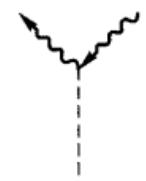
\includegraphics[height=1.55cm]{feyn32-2d.png}} \\[0.2em]
(a) & (b) & (c) & (d)
\end{tabular}
\label{32.2}
\end{equation}

（带有一条或两条波纹线的顶点称作\textbf{不完全顶点}）. 在每个顶点上必须满足“4-动量守恒定律”；因此在顶点b和c上虚线的4-动量与实线的4-动量是相等的，而在顶点d上4-动量等于零. 波纹线永远是图的外线，即与图相连接的只是线的一端，而另一端则保持自由.

进入格林函数$G(P)$定义中的每一个图都有两条4-动量$P$的实外线（入射线和出射线），此外还可以有一定的偶数条波纹外线；各图中的入射外线和出射外线的总数是相同的（以此来表达系统中凝聚体和非凝聚体粒子总数的守恒）. 像费米系统一样（也因为同样的理由——见§13），只有不能分解为两个（或更多个）不相连的子图的图才是允许的. 但与费米系统情况不同的是，这里要改变共同符号的定义规则，按这种规则，$\mathrm{i}G$中所含的图都有相同的符号（即取消48页上的规则3）.

图中每一条虚线在自己的两端都有完全的或不完全的顶点. 但这不会是(32.2d)类型的两个顶点，因为其中连一个实外线也没有，这种图形根本不能与格林函数图相连. 并且也不可能是(32.2d)与(32.2c)［或(32.2d)与(32.2b)］类型的顶点，因为当存在三条波纹外线时，图形中顶点上4-动量的守恒会使得第四条外线的4-动量也变成零，也就是说，我们能得出具有凝聚体全部四条（波纹线的）外线的图形.

然而，按以前叙述的规则建立的微扰论，它的每一级中有相当数目的图总是变成零. 其消失的原因是：理想玻色气体处于基态时不存在非凝聚体粒子. 这点，如果我们仔细考查坐标表象中图的来源，就更清楚了，因为所有$\langle\tilde{\Psi}'^{+}\hat{\Psi}'\rangle$形的收缩都等于零，括号中非凝聚体粒子的湮没算符位于右边，并首先作用在基态上；剩下的只是$\langle\hat{\Psi}'\hat{\Psi}'\rangle$形的收缩\footnote{按同样的理由，两个粒子在真空中散射的某些图也变成零——见§16.}.

例如，“自身封闭”的实线图都将变成零，因为这种线来自非凝聚体粒子密度$\langle\hat{\Psi}'^{+}(t,\bm{r})\hat{\Psi}'(t,\bm{r})\rangle$的收缩. 其次，以虚线封闭的实线图：
\begin{equation*}
\raisebox{-0.3\height}{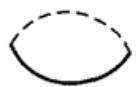
\includegraphics[width=2.6cm]{feyn32-loop1.png}}
\end{equation*}
都等于零. 这种线来自同一个相互作用算符$\hat{V}(t)$里两个$\psi$算符的收缩$\langle\hat{\Psi}'^{+}(t,\bm{r}_{2})\hat{\Psi}'(t,\bm{r}_{1})\rangle$（其中$\hat{\Psi}'^{+}$位于$\hat{\Psi}'$的左边）.

最后，由实线和虚线按一定顺序构成的封闭圈图（而且实线的指向沿整个圈图都相同）所组装的一切图都等于零. 现在我们来画出这类圈图. 在线段的端点旁标出$\psi$算符的时间宗量：
\begin{equation*}
\raisebox{-0.3\height}{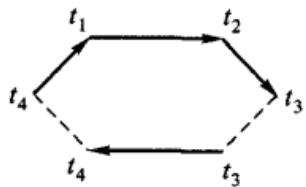
\includegraphics[width=4.2cm]{feyn32-loop2.png}}
\end{equation*}
图中每条虚线端点上的宗量都相同\footnote{应注意：在虚线图的空间-时间表象中，与1和2两点对应的因子是$\mathrm{i}U(X_{1}-X_{2})$，它含有$\delta(t_{1}-t_{2})$.}. 与实线对应的函数$G^{(0)}$的宗量等于差值$t_{2}-t_{1}$，$t_{3}-t_{2}$，$t_{4}-t_{3}$，$t_{1}-t_{4}$；对于任何封闭圈图，这些差值之和等于零，因此即使其中的一个差值是负的，对应的函数$G^{(0)}$也变为零.

上述规则也适用于确定反常格林函数的图，不同的只是：两条实外线，对于函数$F$来说一定是出射线，或对于函数$F^{+}$来讲一定是入射线. 相应地，在这些图中入射波纹线数和出射波纹线数变得不相等了，但要使所有出射线的总数仍等于入射线的总数. 一条实外线描述4-动量$P$，而另一条描述——4-动量$-P$［这里$P$是待求的函数$F(P)$或$F^{+}(P)$的宗量］\footnote{因为$F$是宗量的偶函数，所以$P$的共同符号的选取在这里是无关紧要的.}；根据整个图的“4-动量守恒定律”这两种线的4-动量之和应当等于零.

按图技术计算的格林函数包含两个参数——化学势$\mu$和凝聚体密度$n_{0}$；这两个参数还应当与液体密度$n=N/V$联系起来.

直接由格林函数的定义得出的公式\eqref{31.6}是这三个量之间的一个关系式. 下面得到的方程(33.11)可作为第二关系式，该方程用图技术概念术语明显地表达出化学势$\mu$.

\section{自能函数}

现在我们详细考查格林函数图的结构，为此像在§14中对费米系统的作法一样，在讨论中引入\textbf{自能函数}的概念，即采用的方法是研究一切带有两条实外线的图的集合. 这些图都不可能只截断一条实线就分成两个部分. 但与§14有所不同，就图的外线指向来说，现在可能出现不同的情况：除了带有一条入射线和一条出射线的图外，还存在带有两条出射线或两条入射线的图. 与此相应，就产生了三种自能部分：
\begin{equation}
\raisebox{-0.3\height}{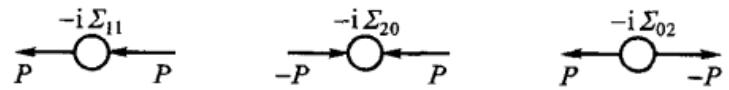
\includegraphics[width=9cm]{feyn33-1.png}}
\label{33.1}
\end{equation}
（这些记号中，$\Sigma$的第一个下标表征入射实外线数，第二个下标表征出射实外线数）. 自能图，除了实外线，一般地说也有波纹线的（凝聚体的）自由端线. 这些端线包含在自能函数的定义中，这里自能函数是以圆圈表示的. 下边我们将会看到，函数$\Sigma_{02}(P)$和$\Sigma_{20}(P)$实际上是相等的：
\begin{equation}
\Sigma_{02}(P)=\Sigma_{20}(P).
\label{33.2}
\end{equation}
还要立即指出，因为$P$和$-P$以对称形式包含在这些函数的定义中，它们是自身宗量的偶函数：
\begin{equation}
\Sigma_{02}(P)=\Sigma_{20}(-P).
\label{33.3}
\end{equation}
作为示例，我们画出函数$\Sigma_{11}$和$\Sigma_{02}$的开头两级微扰论中所有不等于零的图：
\begin{equation}
\raisebox{-0.3\height}{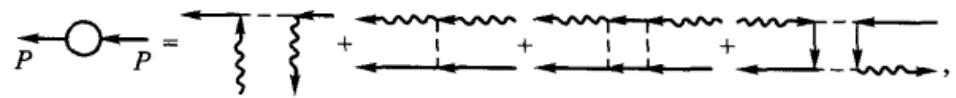
\includegraphics[width=10cm]{feyn33-4.png}}
\label{33.4}
\end{equation}
\begin{equation}
\raisebox{-0.3\height}{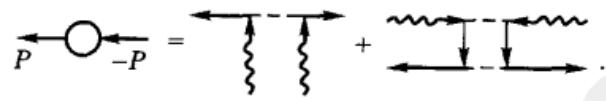
\includegraphics[width=6.5cm]{feyn33-5.png}}
\label{33.5}
\end{equation}

现在我们列出用自能函数表达的精确的函数$G$和$F$的方程.

用微扰论的术语来说，差值$G(P)-G^{(0)}(P)$可用无穷多个链条团之和表达出来，其形状为：
\begin{equation*}
\raisebox{-0.3\height}{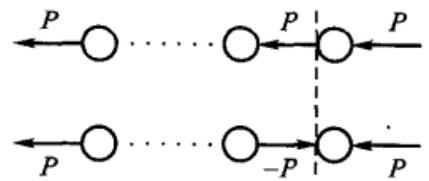
\includegraphics[width=5cm]{feyn33-chG.png}}
\end{equation*}
它们是由不同数量的小圈组成的，圈间用正向和反向（相对于两个端线而言）的箭头以一切可能的方式连接起来. 用同样方法，也可将精确的函数$F$（函数$F^{(0)}\equiv0$）以链条图之和表示出来，链条图中两边上的箭头的指向相反：
\begin{equation*}
\raisebox{-0.3\height}{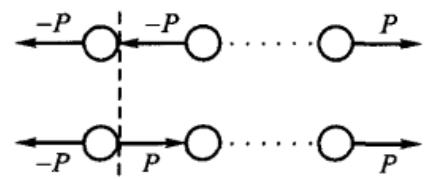
\includegraphics[width=5cm]{feyn33-chF.png}}
\end{equation*}
如果从所有这些链条图中沿竖直虚线所示的地方切断边缘的环节（小圆圈连同箭头），则剩余图的边缘箭头的指向相同的图集合又将与精确的函数$G$一致，而边缘上箭头的指向相反的图集合则与精确的函数$F$一致.

现在我们引入以单向和双向粗箭头表示的这些函数的图记号：
\begin{equation}
\raisebox{-0.3\height}{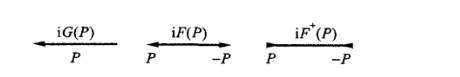
\includegraphics[width=6.5cm]{feyn33-6.png}}
\label{33.6}
\end{equation}
于是，上述论断可写成由骨架图组成的图等式的形式：
\begin{equation}
\raisebox{-0.3\height}{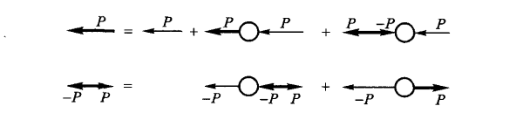
\includegraphics[width=8.5cm]{feyn33-7.png}}
\label{33.7}
\end{equation}
［对比类似的方程(14.4)］. 将这两个等式写成解析形式，得：\footnote{我们也可以写出$G$和$F^{+}$类似的方程组，而该方程组与(33.8)式的区别，只是互换了$\Sigma_{02}$和$\Sigma_{20}$. 因为$F=F^{+}$，所以由此可得出等式(33.2).}
\begin{equation}
\begin{aligned}
&G(P)=\big[1+\Sigma_{11}(P)G(P)+\Sigma_{20}(P)F(P)\big]G^{(0)}(P),\\
&F(P)=G^{(0)}(-P)\big[\Sigma_{11}(-P)F(P)+\Sigma_{02}(P)G(P)\big].
\end{aligned}
\label{33.8}
\end{equation}
求解这两个关于$G$和$F$的方程，并将$G^{(0)}$的表达式\eqref{31.22}代入，便得到所求的函数：
\begin{equation}
\begin{aligned}
&G(P)=\frac{1}{D}\left[\omega+\frac{p^{2}}{2m}-\mu+\Sigma_{11}(-P)\right],\\
&F(P)=-\frac{1}{D}\Sigma_{02}(P),
\end{aligned}
\label{33.9}
\end{equation}
式中
\begin{equation}
\begin{aligned}
D=\big[\Sigma_{02}(P)\big]^{2}-{}\\
-\Big[\Sigma_{11}(P)-\omega-\mathrm{i}0+\frac{p^{2}}{2m}-\mu\Big]
\Big[\Sigma_{11}(-P)+\omega-\mathrm{i}0+\frac{p^{2}}{2m}-\mu\Big].
\end{aligned}
\label{33.10}
\end{equation}

我们强调一下，这些关系式不依赖于自能函数的内部结构，所以也与粒子间具有成对相互作用这一假设无关，因此它们对于任何玻色液体都是正确的.

液体中与动量$\bm{p}$有关的元激发能量，决定于函数$G$和$F$对于变量$\omega$的极点. 当$\bm{p}$很小时，这些元激发是声子，它们的能量同$\bm{p}$一起趋于零. 因此函数\eqref{33.10}当$\bm{p}=0$，$\omega=0$时应变成零. 由此我们求得等式：
\begin{equation*}
\big[\Sigma_{11}(0)-\mu\big]^{2}=\Sigma_{02}^{2}(0),
\end{equation*}
此式作为$\mu$的方程有两个根，其中之一应取
\begin{equation}
\mu=\Sigma_{11}(0)-\Sigma_{02}(0).
\label{33.11}
\end{equation}
实际上，在长波极限下$\psi$算符由(27.2)式给出，非凝聚体部分算符$\hat{\Psi}'=\hat{\Psi}-\sqrt{n_{0}}\approx\mathrm{i}\sqrt{n_{0}}\hat{\Phi}$，因此$\hat{\Psi}'^{*}=-\hat{\Psi}'$，从而$F\approx-G$；后一等式，当取\eqref{33.11}式时恰好得到满足，这时\eqref{33.9}式中的各分子（在$P\to0$的极限情况下）只差一个符号. 等式\eqref{33.11}就是第二关系式（见§32末），它同关系式\eqref{31.6}一起可以把参数$\mu$和$n_{0}$通过液体的密度$n$表达出来.

进一步将表达式\eqref{33.10}按$\omega$和$\bm{p}$展成幂级数，便可决定在宗量$\omega$和$\bm{p}$为小值范围内的格林函数的形式. 这时应该考虑到：标量函数$\Sigma_{11}$和$\Sigma_{02}$可按$\bm{p}^{2}$的幂展开，而对全部宗量为偶函数的$\Sigma_{02}$，它的展开式也只包含变量$\omega$的偶次幂. 将\eqref{33.10}式表为
\begin{equation*}
\begin{aligned}
D=\Big\{\omega+\frac{1}{2}\big[\Sigma_{11}(P)-\Sigma_{11}(-P)\big]\Big\}^{2}-{}\\
-\Big\{\frac{p^{2}}{2m}-\mu+\frac{1}{2}\big[\Sigma_{11}(P)+\Sigma_{11}(-P)\big]\Big\}^{2}
+\Sigma_{02}^{2}(P),
\end{aligned}
\end{equation*}
我们可以立即得出结论：展开式的前几个未消掉的项都具有$D=$常数$(\omega^{2}-u^{2}p^{2}+\mathrm{i}0)^{2}$的形式，其中$u$是一个常数，显然它是液体中的声速. 同时应当指出：由于\eqref{33.11}式，\eqref{33.9}式中的各分子当$\omega,\bm{p}\to0$时只差一个符号，因而求得：
\begin{equation*}
G=-F=\frac{\text{常数}}{\omega^{2}-u^{2}p^{2}+\mathrm{i}0}.
\end{equation*}
根据这个格林函数，算出$\bm{p}$很小时的粒子动量分布$N(\bm{p})$，并把它与我们已知的分布(27.7)对比，则能确定出分子中的常数值. 积分
\begin{equation*}
N(\bm{p})=\mathrm{i}\lim_{t\to-0}\int_{-\infty}^{\infty}G(\omega,\bm{p})\,\mathrm{e}^{-\mathrm{i}\omega t}\frac{\mathrm{d}\omega}{2\pi}
\end{equation*}
［对比(7.23)式］可采用在上半平面内以无穷远的半圆周封闭积分围道的方法计算出来（对比§7最末的讨论），该积分相应地决定于$\omega=-up+\mathrm{i}0$极点上的留数. 最后我们得到$N(\bm{p})=$常数$/2up$，将它与(27.7)式对比，即得出常数$=n_{0}mu^{2}/n$. 因此，最终求得$\omega$和$\bm{p}$为很小值时格林函数表为下式：
\begin{equation}
G=-F=\frac{n_{0}mu^{2}}{n(\omega^{2}-u^{2}p^{2}+\mathrm{i}0)}.
\label{33.12}
\end{equation}

应当指出，在精确到可差归一化系数的情况下，该函数与声子场格林函数相等（见§31中的习题），这个结论是十分自然的，因为在$\omega$和$\bm{p}$为很小值的范围内，玻色液体中的全部元激发都是声子.

最后，我们演示所得公式用于研究§25中近理想玻色气体粒子成对相互作用的模型. 在微扰论的一级近似下，$\Sigma_{11}$和$\Sigma_{02}$决定于\eqref{33.4}的前两个图及\eqref{33.5}的第一个图. 将它们写成解析形式，得到：
\begin{equation*}
\Sigma_{11}=n_{0}[U_{0}+U(\bm{p})],\quad\Sigma_{02}=n_{0}U(\bm{p}).
\end{equation*}
在同样的精确度下，这两个公式中的凝聚体密度$n_{0}$可以换成气体的总密度$n$. 在§25中已指出，在这个模型中气体粒子的动量可认为是很小的，与此相应，各傅里叶分量$U(\bm{p})$可用它们在$\bm{p}=0$时的值$U_{0}$来代换. 于是
\begin{equation}
\Sigma_{11}=2nU_{0},\quad\Sigma_{02}=nU_{0}.
\label{33.13}
\end{equation}
将这两个表达式代入\eqref{33.11}式，得出$\mu=nU_{0}$，它与(25.6)式符合. 若代入(33.9—33.10)式，则得到格林函数的下列两个公式：
\begin{equation}
\begin{aligned}
&G(\omega,\bm{p})=\frac{\omega+p^{2}/2m+nU_{0}}{\omega^{2}-\varepsilon^{2}(\bm{p})+\mathrm{i}0},\\
&F(\omega,\bm{p})=\frac{-nU_{0}}{\omega^{2}-\varepsilon^{2}(\bm{p})+\mathrm{i}0},
\end{aligned}
\label{33.14}
\end{equation}
式中
\begin{equation*}
\varepsilon(\bm{p})=\left[\left(\frac{p^{2}}{2m}\right)^{2}+\frac{p^{2}}{m}nU_{0}\right]^{1/2}.
\end{equation*}
从这两个函数分母的形式显然可看出$\varepsilon(p)$就是元激发能量，这符合以前用另一种方法得到的结果(25.10—25.11).

\section{准粒子的裂变}

量子液体中一个准粒子具有有限寿命（发生衰减），与它同其它准粒子发生碰撞或它自发裂变成两个（或更多个）新的准粒子有关. 当温度$T\to0$时，衰减的第一个原因消失了（因为碰撞概率跟准粒子数密度一起趋于零），这样，衰减只能由准粒子的裂变才会发生.

现在来研究动量为$\bm{p}$的准粒子裂变为二的情况. 如果$\bm{q}$是所出现的准粒子之一的动量，则另一个准粒子的动量为$\bm{p}-\bm{q}$，能量守恒定律给出如下条件：
\begin{equation}
\varepsilon(p)=\varepsilon(q)+\varepsilon(|\bm{p}-\bm{q}|).
\label{34.1}
\end{equation}
可以看出，在$\bm{p}$值的某一范围内，这个等式对于任何$\bm{q}$都不满足；这时，这个范围内的准粒子根本不会衰减（当然，假如也不能裂变为更多的准粒子）.

随着$\bm{p}$的改变，当$p=p_{c}$（裂变阈）时，会首次出现方程\eqref{34.1}的根. 这时将发生衰减.

首先应当指出：在$p=p_{c}$这一点，方程\eqref{34.1}的右边作为$\bm{q}$的函数是具有极值的. 事实上，令$\varepsilon(\bm{q})+\varepsilon(|\bm{p}-\bm{q}|)$在给定$\bm{p}$值时的极值是$E(p)$（为了明确起见，我们将把它看作是极小值）. 于是，方程
\begin{equation*}
\varepsilon(p)-E(p)=\varepsilon(q)+\varepsilon(|\bm{p}-\bm{q}|)-E(p)
\end{equation*}
的右边是非负的. 因此，当$\bm{p}$值满足$\varepsilon(p)-E(p)<0$时，方程显然没有根；而只在$p=p_{c}$这一点才有根出现，在该点上$\varepsilon(p_{c})=E(p_{c})$.

将方程\eqref{34.1}表为对称形式：
\begin{equation*}
\varepsilon(p)=\varepsilon(q_{1})+\varepsilon(q_{2}),\quad
\bm{q}_{1}+\bm{q}_{2}=\bm{p},
\end{equation*}
我们发现，方程右边的极值条件可以写成$\partial\varepsilon/\partial\bm{q}_{1}=\partial\varepsilon/\partial\bm{q}_{2}$或
\begin{equation}
\bm{v}_{1}=\bm{v}_{2},
\label{34.2}
\end{equation}
也就是说，在阈点上两个裂变出的准粒子具有相同的速度. 这里可以分为以下几种情况（Л.\,П.\,皮塔耶夫斯基，1959）.

a) 当$p=p_{0}$时，玻色液体中准粒子的速度等于零，而$p_{0}$对应于图2曲线上旋子的极小值. 因此，如果$\bm{v}_{1}=\bm{v}_{2}=0$，其意思是指：在阈点上准粒子裂变为两个动量为$\bm{p}_{0}$、能量为$\varDelta$的旋子. 相应地，发生裂变的准粒子的能量$\varepsilon(p_{c})=2\varDelta$，而它的动量$p_{c}$是以$\bm{p}_{c}=\bm{p}_{01}+\bm{p}_{02}$，即$2p_{0}\cos\theta=p_{c}$这一条件与$\bm{p}_{0}$联系起来，这里$2\theta$是两个旋子飞出的夹角. 由此得出，在所有情况下必有：
\begin{equation}
p_{c}<2p_{0}.
\label{34.3}
\end{equation}

b) 假若速度$\bm{v}_{1}=\bm{v}_{2}\neq0$，并且与它们相应的动量$\bm{q}_{1}$和$\bm{q}_{2}$是有限的，其意思是指：在阈点上的裂变产生两个具有共线（平行或反平行的）动量的准粒子\footnote{由于液体是各向同性的，准粒子动量$\bm{p}$及其速度$\bm{v}=\partial\varepsilon/\partial\bm{p}$取向共线，但方向可能相同也可能相反.}.

c) 如果速度$\bm{v}_{1}$和$\bm{v}_{2}$均不为零，但动量之一（譬如说$\bm{q}_{1}$）在阈点附近趋于零，那么相应于该动量的准粒子是声子，并且速度$\bm{v}_{1}=u$. 此时可有这样的阈点，超过此点便可以由准粒子产生声子. 在阈点上声子的能量等于零，准粒子速度刚刚达到声速（速度$\bm{v}_{1}=\bm{v}_{2}=u$全相同）.

d) 最后还有一种特殊情况，即一个声子裂变成两个声子，而且阈点就是能谱的始点$p=0$. 但是这种裂变只当能谱起始一段（声子段）的曲率具有确定的符号［应为$\mathrm{d}^{2}\varepsilon(p)/\mathrm{d}p^{2}>0$］时才可能，也就是说$\varepsilon(p)$曲线必须从起始的切线$\varepsilon=up$起向上弯曲. 这不难证明，现在将这一段能谱表为如下形式：
\begin{equation}
\varepsilon(p)\approx up+\alpha p^{3},
\label{34.4}
\end{equation}
该式除线性项以外也计入了按小动量的幂展开的下一项\footnote{由声振动的色散方程可将频率平方$\omega^{2}$确定为波矢量函数. 与此相应，将声子能量的平方$\varepsilon^{2}(p)$按动量$\bm{p}$的幂作正则展开；由于液体是各向同性的，所以从$\sim\bm{p}^{2}$项开始应按$\bm{p}^{2}$的幂展开. 因而，函数$\varepsilon(p)$本身的展开式便含有$p$的奇次幂.}. 于是由能量守恒方程\eqref{34.1}得出：
\begin{equation*}
u\big(p-q-|\bm{p}-\bm{q}|\big)
=-\alpha\big(p^{3}-q^{3}-|\bm{p}-\bm{q}|^{3}\big).
\end{equation*}
在阈点附近与准粒子起始动量$\bm{p}$成小角$\theta$的方向射出一个声子；在方程的左边，有：
\begin{equation}
p-q-|\bm{p}-\bm{q}|\approx-\frac{pq}{p-q}\big(1-\cos\theta\big).
\label{34.5}
\end{equation}
在方程的右边，只要令$|\bm{p}-\bm{q}|\approx p-q$，就可以求得：
\begin{equation}
u\big(1-\cos\theta\big)=3\alpha(p-q)^{2},
\label{34.6}
\end{equation}
由此可见，应当是$\alpha>0$.

我们在下面（§35）将会看到：在a)和b)两种情况，函数$\varepsilon(p)$不可能在阈点以后延拓，因此这一点是能谱的终点. 但在c)和d)两种情况，辐射长波声子的准粒子，其裂变会导致弱衰减的出现，这可以借助微扰论来确定\footnote{上面所列举的各种情况中，究竟哪几种实际上能够实现，这有赖于准粒子谱$\varepsilon(p)$曲线的具体走向. 关于液氦($^{4}$He)的一些实验资料，证明了在压强小于15个大气压时有开始不大一段声子谱存在，在这一段里具有第d)种情况的不稳定性. 液氦谱终止于第a)种情况的点上.}.

现在我们来计算由一个声子裂变成两个声子的衰减（第d种情况）. 由(24.12)式给出的哈密顿量的各三次项中，都有这种过程的矩阵元. 对于由动量为$\bm{p}$的一个声子的初态$(i)$到动量为$\bm{q}_{1}$和$\bm{q}_{2}$的两个声子的末态$(f)$的跃迁，微扰算符的矩阵元等于
\begin{equation}
V_{fi}=\frac{1}{\mathrm{i}}\delta(\bm{p}-\bm{q}_{1}-\bm{q}_{2})
\frac{3!\,(2\pi\hbar)^{3}}{2\,(2V)^{3/2}}
\left(\frac{u}{\rho}pq_{1}q_{2}\right)^{1/2}
\left\{1+\frac{\rho^{2}\,\mathrm{d}u^{2}}{3u^{2}\,\mathrm{d}\rho\,\rho}\right\}
\label{34.7}
\end{equation}
（略去了无微扰密度$\rho_{0}$的下标0）. 注意其中有$(pq_{1}q_{2})^{1/2}$这一因子；由于它很小（指的是长波声子的裂变），因而保证可以运用微扰论\footnote{计算矩阵元(34.7)时，应考虑到：声子算符$\hat{c}_{\bm{p}}$和$\hat{c}^{+}_{\bm{p}}$中的每一个都可以从$\hat{\rho}'$或$\bm{v}$的三个因子中任选一个；因此出现因子3!. (34.7)式中的$\delta$函数是由积分$\exp[\mathrm{i}(\bm{p}-\bm{q}_{1}-\bm{q}_{2})\bm{r}/\hbar]$因子而产生的. 最后注意，$\bm{p}$，$\bm{q}_{1}$和$\bm{q}_{2}$的方向几乎重合.}.

在1 s内裂变的微分概率由下列公式给出：
\begin{equation*}
\mathrm{d}\omega=\frac{2\pi}{\hbar}|V_{fi}|^{2}\delta(E_{f}-E_{i})
\frac{V^{2}\,\mathrm{d}^{3}q_{1}\,\mathrm{d}^{3}q_{2}}{(2\pi\hbar)^{6}}.
\end{equation*}
［见第三卷(43.1)式］. 把\eqref{34.7}式代入上式时将出现$\delta$函数的平方；应把它理解为\footnote{实际上，$\delta$函数$\delta(\bm{k})$产生于积分$\int\mathrm{e}^{\mathrm{i}\bm{k}\cdot\bm{r}}\,\mathrm{d}^{3}r/(2\pi)^{3}$. 如果计算$\bm{k}=0$时的另一个同样的积分（因为已有了一个$\delta$函数），并且遍及有限体积$V$进行积分，则得到$V/(2\pi)^{3}$；这就是公式(34.8)所表达的.}
\begin{equation}
\big[\delta(\bm{p}-\bm{q}_{1}-\bm{q}_{2})\big]^{2}
=\frac{V}{(2\pi\hbar)^{3}}\,\delta(\bm{p}-\bm{q}_{1}-\bm{q}_{2}),
\label{34.8}
\end{equation}
剩下的一个$\delta$函数被对$\mathrm{d}^{3}q_{2}$的积分消掉了；这里也取$E_{i}=up$，$E_{f}=u(q_{1}+q_{2})$，我们得到：
\begin{equation*}
w=\frac{1}{2}\left\{1+\frac{\rho^{2}\,\mathrm{d}u^{2}}{3u^{2}\,\mathrm{d}\rho\,\rho}\right\}^{2}
\cdot\frac{9\pi}{4\hbar\rho}\int pq_{1}(p-q_{1})\,
\delta\big(p-q_{1}-|\bm{p}-\bm{q}_{1}|\big)
\frac{\mathrm{d}^{3}q_{1}}{(2\pi\hbar)^{3}}
\end{equation*}
（当分别对$\mathrm{d}^{3}q_{1}$和$\mathrm{d}^{3}q_{2}$积分时，考虑两个声子的全同性，答案应除以2）. 最后，把$\delta$函数的宗量表达成\eqref{34.5}式，并对$\mathrm{d}^{3}q_{1}=2\pi q_{1}^{2}\,\mathrm{d}q_{1}\,\mathrm{d}\cos\theta$（在$q_{1}\leqslant p$的区域）进行积分，可求得裂变的总概率：
\begin{equation}
w=\frac{3p^{5}}{320\pi\rho\hbar^{4}}
\left\{1+\frac{\rho^{2}}{3u^{2}}\frac{\mathrm{d}u^{2}}{\mathrm{d}\rho\,\rho}\right\}^{2},
\label{34.9}
\end{equation}
声子的衰减系数$\gamma\equiv-\mathrm{Im}\ \varepsilon=\hbar w/2$. 其中，对于近理想玻色气体来说，根据(25.11)式，$u^{2}/\rho\approx4\pi\hbar^{2}a/m^{3}$这一数值与密度无关. 在这种情况下
\begin{equation}
\gamma=\frac{3p^{5}}{640\pi\hbar^{3}\rho}
\label{34.10}
\end{equation}
（С.\,Т.\,Беляев，1958）.

对于第c)种情况在阈点附近准粒子辐射声子的过程来说，微扰算符的形式可借助研究声波中准粒子能量的改变来确定. 这种能量改变由两部分组成：
\begin{equation*}
\delta\varepsilon(\bm{p})=\frac{\partial\varepsilon}{\partial\rho}\rho'+\bm{v}\cdot\bm{p}.
\end{equation*}
第一项与液体密度的变化有关，准粒子能量依赖于作为参量的液体密度. 第二项（其中$\bm{v}$是声波中液体的速度）是由于液体宏观运动而形成的准粒子能量的改变；因为在阈点附近辐射出的声子波长大于准粒子的波长，所以可以认为：准粒子处于均匀液流之中，于是准粒子能量的改变就可如§23初段所述给以确定. 在$\delta\varepsilon$中使$\bm{v}=\nabla\varphi$，将$\rho'$换成二次量子化算符(24.10)，并将$\bm{p}$换成准粒子动量算符$\hat{\bm{p}}=-\mathrm{i}\hbar\nabla$，即可得到微扰算符：
\begin{equation}
\hat{V}=\frac{\partial\varepsilon}{\partial\rho}\hat{\rho}'
+\frac{1}{2}\big(\hat{\bm{v}}\cdot\hat{\bm{p}}+\hat{\bm{p}}\cdot\hat{\bm{v}}\big)
\label{34.11}
\end{equation}
（在第二项中把乘积加以对称化，以使其成为厄米形式）. 其次，可像上面处理声子裂变一样来计算声子辐射的概率（见习题）.

\begin{xiti}

1. 试求动量为$p$（接近于阈值$p_{c}$）的准粒子辐射声子的概率，这时准粒子速度达到声速.

{\heiti 解：}准粒子在动量为$\bm{p}$和$\bm{p}'$两个状态（平面波）间跃迁，同时产生一个声子（动量为$\bm{q}$），对这一情况取算符\eqref{34.11}的矩阵元. 在阈点附近，声子的动量$q\ll p_{c}$，而$\bm{q}$的方向几乎与$\bm{p}$的方向重合\footnote{为了明确起见，我们研究声子恰好以这个方向（而不是相反方向）被辐射时的情况. 对此，函数$\varepsilon(p)$在阈点附近应有如下形式：
\begin{equation*}
\varepsilon(\bm{p})\approx\varepsilon(p_{c})+(p-p_{c})u+\alpha(p-p_{c})^{2}
\end{equation*}
（线性项的符号为正）. 根据能量守恒定律不难证明：当$\alpha>0$以及$p>p_{c}$时才能发生声子辐射；辐射出的声子动量取遍$0\leqslant q\leqslant 2(p-p_{c})$间隔内的一切值.}. 考虑到这一点，即可求出：
\begin{equation*}
V_{fi}=-\mathrm{i}(2\pi\hbar)^{3}\delta(\bm{p}-\bm{q}_{1}-\bm{q}_{2})
\frac{A}{V^{3/2}}\left(\frac{qu}{2\rho}\right)^{1/2},
\end{equation*}
式中
\begin{equation*}
A=p_{c}+\frac{\rho}{u}\frac{\partial\varepsilon}{\partial\rho}\bigg|_{p=p_{c}},
\end{equation*}
因而声子辐射的微分概率为
\begin{equation*}
\mathrm{d}w=\frac{\pi qu}{\hbar\rho}A^{2}
\delta\big[\varepsilon(p)-\varepsilon(|\bm{p}-\bm{q}|)-uq\big]
\frac{\mathrm{d}^{3}q}{(2\pi\hbar)^{3}}
\end{equation*}
（动量的$\delta$函数已被对$\mathrm{d}^{3}\bm{p}'$的积分消掉）. 把$\delta$函数的宗量写成近似形式$-uq(1-\cos\theta)$并对$\mathrm{d}^{3}\bm{q}$进行积分，则得：
\begin{equation*}
w=\frac{2A^{2}(p-p_{c})^{3}}{3\pi\rho\hbar^{4}}.
\end{equation*}

2. 初速度为$\bm{v}$的中子在液体内散射. 试求此时可以产生动量为$\bm{p}$，能量为$\varepsilon(p)$的激发的条件.

{\heiti 解：}在所考察的过程中能量和动量守恒可以写成如下的方程（$m$为中子质量，$\bm{P}$为其初动量）：
\begin{equation*}
\frac{P^{2}}{2m}-\frac{(P-\bm{p})^{2}}{2m}=\varepsilon(\bm{p}),
\end{equation*}
或
\begin{equation*}
Vp\cos\theta=\varepsilon(p)+\frac{p^{2}}{2m},
\end{equation*}
这里$\theta$是$\bm{P}$，$\bm{p}$间夹角，于是待求的条件为
\begin{equation*}
V\geqslant\frac{\varepsilon(p)}{p}+\frac{p}{2m}.
\end{equation*}

\end{xiti}

\section{能谱在其终点附近的性质}

这一节我们将研究在元激发裂变成两个准粒子的阈点附近玻色液体谱的性质，但这两个准粒子当中一个也不是声子［§34中的a)和b)两种情况］\footnote{这一节的内容属于Л.\,П.\,皮塔耶夫斯基的工作(1959).}. 与产生声子的裂变相反，对于a)，b)两种情况微扰论是不适用的，并且研究这两种裂变时需要阐明液体的格林函数在阈点处的奇异性质. 另一方面，使我们只对这些奇异性感兴趣这一事实，便允许更大程度地使用图解法，因而简化了计算过程. 比如说，可以不必区别$G$和$F$这两个函数（因为它们的解析性质是相同的），因而可以认为只存在一种格林函数；若考虑$G$和$F$之间的区别，只会使方程中出现若干个同类项（按其解析性质划分），但这并不影响所得的结果.

我们感兴趣的格林函数的奇异性与一个准粒子裂变成另外两个准粒子有关，这一事实用图技术的术语来说，就是指奇异性出自如下形状的图：
\begin{equation}
\raisebox{-0.3\height}{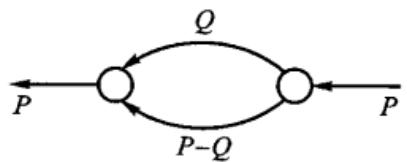
\includegraphics[width=5.5cm]{feyn35-1.png}}
\label{35.1}
\end{equation}
这些图可以切断两条实线而被截开，也就是说，各图本身包含双粒子的中间态. 在这些图中对中间4-动量$Q=(q_{0},\bm{q})$进行积分. 并且就产生奇异性来说，$Q$和$P-Q$的值域起决定性作用，而裂变出的准粒子（裂变产物）就以这些动量在阈点附近产生出来. 对于所要阐明的理论来说下述论断是重要的：对于格林函数$G(Q)$，这个4-动量值域并不是奇异的，因为在这个值域内$G(Q)$具有通常的极点的形式：
\begin{equation}
G(\bm{Q})\equiv G(q_{0},\bm{q})\propto\big[q_{0}-\varepsilon(\bm{q})+\mathrm{i}0\big]^{-1},
\label{35.2}
\end{equation}
其中函数$\varepsilon(q)$是裂变出的准粒子能量，它不具有奇异性. 这个值域的物理特殊性，只在于其中一个准粒子能和另一个准粒子“粘”在一起；但这个过程在绝对零度时是不可能发生的，因为这时不存在真实的激发. 格林函数的奇异域只是原来的准粒子裂变阈附近的一些$P$值［图\eqref{35.1}的外线］.

图\eqref{35.1}中的两条连接线对应于因子$G(Q)G(P-Q)$，而对$Q$进行积分. 这里，因为只有$Q$的小值域是重要的，所以图中其余的因子在求积分时可以当作常量，并等于它们在阈值$Q=Q_{c}$时的值\footnote{对这个论点应该作明确解释. 因为，因子$G(Q)G(P-Q)$与决定$(\bm{p},\bm{q})$平面位置的角$\varphi$无关. 所以对$\mathrm{d}\varphi$求积分归结为将被积式其余部分对$\varphi$求平均，此后$\mathrm{d}^{4}Q$便可以理解为$2\pi q^{2}\,\mathrm{d}q_{0}\,\mathrm{d}q\,\mathrm{d}\cos\theta$. 在这种对$\mathrm{d}^{4}Q$的积分中，小值域恰恰是重要的. 对于下面计算的其它类似场合也应注意此点.}. 因此，在图中出现用积分表达的因子：
\begin{equation*}
\Pi(P)=\frac{\mathrm{i}}{(2\pi)^{4}}\int
\frac{\mathrm{d}^{4}Q}{\big[q_{0}-\varepsilon(\bm{q})+\mathrm{i}0\big]
\big[\omega-q_{0}-\varepsilon(|\bm{p}-\bm{q}|)+\mathrm{i}0\big]}
\end{equation*}
式中$P=(\omega,\bm{p})$. 借助于在复数$q_{0}$的一个半平面内用无穷远半圆封闭积分围道的方法来完成对$\mathrm{d}q_{0}$的积分，于是得出：
\begin{equation}
\Pi(P)=\frac{1}{(2\pi)^{3}}\int
\frac{\mathrm{d}^{3}q}{\omega-\varepsilon(\bm{q})-\varepsilon(|\bm{p}-\bm{q}|)+\mathrm{i}0}
\label{35.3}
\end{equation}

下面我们还要分析这个积分，现在需要用它将所求的精确函数$G(P)$表达出来，为此应把所有(35.1)形的图累加起来.

函数$G(P)$可以写成戴森图方程：
\begin{equation}
\raisebox{-0.3\height}{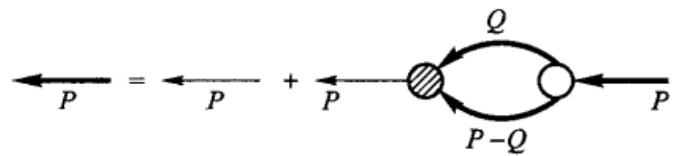
\includegraphics[width=8cm]{feyn35-4.png}}
\label{35.4}
\end{equation}
这里粗线表示精确函数$\mathrm{i}G$，细线表示这个函数的“非奇异”部分，后者由“切断两条线”而不能截开的图形的集合所定义的. \eqref{35.4}式右边第二项表示(35.1)图形的集合. 这时白小环代表精确的“三端”顶角函数［用$\Gamma(Q,P-Q,P)$标记］，阴影小环代表该函数的非奇异部分，这个部分已经消去了因切断两条实线而被截开的图\footnote{这里所说的情况与量子电动力学中的戴森方程相似（见第四卷§107）：同那里一样，所有必要的图的集合都是只修正一个顶角函数而得到的.}. 如上所述，对$\mathrm{d}^{4}Q$求积分会出现因子$\Pi(P)$，并且图中其余的因子可代之以它们的$Q=Q_{c}$时的值. 所以等式\eqref{35.4}就是：
\begin{equation}
G(P)=a(P)+b(P)G(P)\Gamma_{c}(P)\Pi(P)
\label{35.5}
\end{equation}
式中$\Gamma_{c}(P)=\Gamma(Q_{c},P-Q_{c},P)$，而$a(P)$，$b(P)$是$P=P_{c}$阈点附近的两个正则函数.

在\eqref{35.5}式中出现的$G$和$\Gamma_{c}$是两个奇异函数，为了通过$\Pi$将它们表达出来，还需要有一个方程. 注意，将精确的顶角函数$\Gamma$表示成“梯形”级数
\begin{equation*}
\raisebox{-0.3\height}{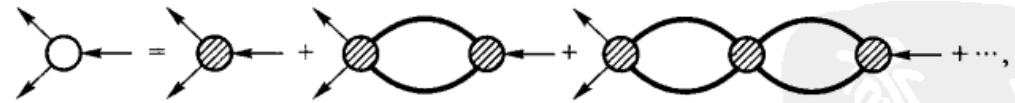
\includegraphics[width=10.5cm]{feyn35-lad1.png}}
\end{equation*}
我们就得到这一方程，上列级数与四端顶角函数的级数(17.3)类似. 级数之和可给出方程：
\begin{equation*}
\raisebox{-0.3\height}{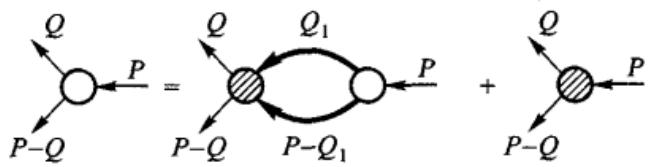
\includegraphics[width=8cm]{feyn35-lad2.png}}
\end{equation*}
［比较(17.4)］；当$Q\approx Q_{c}$时，这一方程可给出如下的解析式：
\begin{equation*}
\Gamma_{c}(P)=c(P)+d(P)\Pi(P)\Gamma_{c}(P),
\end{equation*}
式中$c(P)$，$d(P)$是正则函数. 现在从上述两个方程中消去$\Gamma_{c}$，我们便得到所求的格林函数通过$\Pi$的表达式：
\begin{equation}
G^{-1}(P)=\frac{A(P)\Pi(P)}{1+B(P)\Pi(P)}+C(P),
\label{35.6}
\end{equation}
这里$A$，$B$，$C$也都是$P=P_{c}$附近的正则函数.

对不同类型的准粒子裂变作进一步计算有不同的情况.

\par\medskip\noindent{\heiti a)\ 裂变成两个旋子的阈}\par\smallskip

在这种情况下，阈点附近裂变粒子的能量$\varepsilon(\bm{q})$由公式(22.6)给出，于是\eqref{35.3}式的积分取如下形式：
\begin{equation}
\begin{aligned}
\Pi(\omega,\bm{q})={}\\
=\int\Big\{\omega-2\varDelta-\frac{1}{2m^{*}}
\big[(\bm{q}-\bm{p}_{0})^{2}+(|\bm{p}-\bm{q}|-\bm{p}_{0})^{2}\big]\Big\}^{-1}
\frac{\mathrm{d}^{3}q}{(2\pi)^{3}}.
\end{aligned}
\label{35.7}
\end{equation}
为求积分我们引入两个新的变量$q'_{z}$，$q'_{\rho}$，根据定义，有
\begin{equation*}
\begin{aligned}
&q_{x}=(p_{0}\sin\theta+q'_{\rho})\cos\varphi,\quad
q_{y}=(p_{0}\sin\theta+q'_{\rho})\sin\varphi,\\
&q_{z}=p_{0}\cos\theta+q'_{z},
\end{aligned}
\end{equation*}
并且$z$轴沿$\bm{p}$的方向，角$\theta$决定于等式$2p_{0}\cos\theta=p$. 在阈点附近$q'_{z}$，$q'_{\rho}$很小，因而以所需的精确度有：
\begin{equation*}
\begin{aligned}
&q\approx p_{0}+q'_{\rho}\sin\theta+q'_{z}\cos\theta,\\
&|\bm{p}-\bm{q}|\approx p_{0}+q'_{\rho}\sin\theta-q'_{z}\cos\theta,\\
&\mathrm{d}^{3}q\approx p_{0}\sin\theta\,\mathrm{d}q'_{\rho}\,\mathrm{d}q'_{z}\,\mathrm{d}\varphi,
\end{aligned}
\end{equation*}
这时\eqref{35.7}式中花括号内的表达式取下列形式：
\begin{equation*}
\left\{\omega-2\varDelta-\frac{1}{m^{*}}
\big(q_{\rho}^{\prime2}\sin^{2}\theta+q_{z}^{\prime2}\cos^{2}\theta\big)\right\}.
\end{equation*}
再作一次变量代换：
\begin{equation*}
q'_{\rho}\sin\theta=\sqrt{m^{*}}\,\rho\cos\psi,\quad
q'_{z}\cos\theta=\sqrt{m^{*}}\,\rho\sin\psi,
\end{equation*}
然后对$\psi$积分，可求得：
\begin{equation*}
\Pi(\omega,\bm{p})=-\frac{m^{*}p_{0}}{2\pi\cos\theta}
\int\frac{\rho\,\mathrm{d}\rho}{-\omega+2\varDelta+\rho^{2}}.
\end{equation*}
$\rho$很大时，式中积分的发散性只与所作的若干忽略有关，因而是无关重要的；当$\rho^{2}$的某一值$\gg|2\varDelta-\omega|$时，积分的截断只对$\Pi$的正则部分有贡献. 我们感兴趣的这个函数的奇异部分产生于积分下限附近区域，于是我们求得奇异部分：
\begin{equation}
\Pi\propto\ln\frac{1}{2\varDelta-\omega}.
\label{35.8}
\end{equation}
当$2\varDelta-\omega$值很小时，这个对数很大；把\eqref{35.8}式代入\eqref{35.6}式并按对数的负幂次展开，我们得到：
\begin{equation*}
G^{-1}(\omega,p)=b+c\ln^{-1}\frac{a}{2\varDelta-\omega},
\end{equation*}
式中$a$，$b$，$c$是$\omega$和$p$的新正则函数. 在阈点$(p=p_{c})$发生裂变的准粒子能量等于$2\varDelta$. 因为准粒子能量决定于函数$G^{-1}$的零点，就是说$G^{-1}(2\varDelta,p_{c})=0$，对此也应有$b(2\varDelta,p_{c})=0$. 但是，将正则函数$b(\omega,p)$按差$p-p_{c}$与差$\omega-2\varDelta$的整数幂展开；将正则函数$a(\omega,p)$和$c(\omega,p)$也换成它们在阈点上的值，最后我们得到阈点附近区域内格林函数的如下表达式：
\begin{equation}
G^{-1}(\omega,p)=\beta\left[p-p_{c}+\alpha\ln^{-1}\frac{a}{2\varDelta-\omega}\right].
\label{35.9}
\end{equation}
其中$a$，$\alpha$，$\beta$是常数.

令这个表达式等于零，我们即得到阈点附近能谱$\varepsilon(p)$的形式. 假如不可裂变区域位于$p<p_{c}$，$\varepsilon<2\varDelta$的范围，则常数$\alpha$和$a$必为正数，因而方程$G^{-1}=0$这里具有不衰减的解：
\begin{equation}
\varepsilon=2\varDelta-a\exp\left(-\frac{\alpha}{p_{c}-p}\right).
\label{35.10}
\end{equation}
我们看到，能谱曲线终于阈点，并且在该点具有无限阶的水平切线. 但在$p>p_{c}$的区域内，方程$G^{-1}=0$既没有实数解，也没有$p\approx p_{c}$时$\varepsilon\approx2\varDelta$的复数解. 就此意义来说，能谱曲线根本不可能延拓到阈点之后，而只能终止于该点\footnote{在123页的注解中已经指出：在液氦的情况下，能谱恰好终止于这种点（图2中的曲线具有水平切线并逐渐接近于直线$\varepsilon=2\varDelta$）.}.

\par\medskip\noindent{\heiti b)\ 裂变成具有平行动量的两个准粒子的阈}\par\smallskip

因为在阈点（当$p=p_{c}$时），表达式$\varepsilon(\bm{q})+\varepsilon(|\bm{p}-\bm{q}|)$作为$\bm{q}$的函数应具有极小值，所以在阈点附近该式有如下形式：
\begin{equation}
\begin{aligned}
&\varepsilon(\bm{q})+\varepsilon(|\bm{p}-\bm{q}|)={}\\
&=\varepsilon_{c}+v_{c}(p-p_{c})
+\alpha(\bm{q}-\bm{q}_{0})^{2}
+\beta(\bm{q}-\bm{q}_{0},\bm{p}_{c})^{2},
\end{aligned}
\label{35.11}
\end{equation}
式中$\alpha$，$\beta$是常数；$v_{c}$是在阈点因裂变而产生的每个准粒子的速度，$\bm{q}_{0}$是一个准粒子的动量. 将\eqref{35.11}式代入\eqref{35.3}式，并按照
\begin{equation*}
\bm{\rho}=\bm{q}-\bm{q}_{0},\quad
\bm{\rho}\,\bm{p}_{c}=\rho p_{c}\cos\psi
\end{equation*}
引入新的积分变量，得：
\begin{equation*}
\Pi(\omega,p)=\frac{1}{(2\pi)^{2}}\int
\frac{\rho^{2}\,\mathrm{d}\rho\,\mathrm{d}\cos\psi}
{\varepsilon-\varepsilon_{c}-v_{c}(p-p_{c})-\alpha\rho^{2}-\beta\rho^{2}p_{c}^{2}\cos^{2}\psi}
\end{equation*}
这个积分在阈点具有平方根的奇异性：
\begin{equation}
\Pi\propto\big[v_{c}(p-p_{c})-(\varepsilon-\varepsilon_{c})\big]^{1/2}.
\label{35.12}
\end{equation}
把上式代入\eqref{35.6}式，我们便求得阈点附近区域内的格林函数：
\begin{equation*}
G^{-1}(\omega,p)=A(\omega,p)+B(\omega,p)
\big[v_{c}(p-p_{c})-(\omega-\varepsilon_{c})\big]^{1/2}.
\end{equation*}
因为$G^{-1}(\varepsilon_{c},p_{c})=0$，而$A$和$B$是正则函数，所以将$A$，$B$按$p-p_{c}$和$\omega-\varepsilon_{c}$的幂展开，最终求得：
\begin{equation}
G^{-1}\propto\big[v_{c}(p-p_{c})-(\omega-\varepsilon_{c})\big]^{1/2}
+\big[a(p-p_{c})+b(\omega-\varepsilon_{c})\big],
\label{35.13}
\end{equation}
式中$a$，$b$是常数.

能谱的形状决定于方程$G^{-1}(\varepsilon,\bm{p})=0$. 现在我们来寻求该方程形如$\varepsilon-\varepsilon_{c}=v_{c}(p-p_{c})+$常数$(p-p_{c})^{2}$的解，为使方程当$p<p_{c}$时有解，必须有$a+bv_{c}>0$，于是
\begin{equation}
\varepsilon=\varepsilon_{c}+v_{c}(p-p_{c})-(a+bv_{c})^{2}(p-p_{c})^{2}.
\label{35.14}
\end{equation}
在同样条件下，在$p>p_{c}$的区域内，方程$G^{-1}=0$不具有$p\approx p_{c}$时$\varepsilon\approx\varepsilon_{c}$的解. 因此，在这种情况下能谱也止于阈点.

\section*{§35*\quad 二维系统的超流性}
\phantomsection
\addcontentsline{toc}{section}{\numberline {§35*}二维系统的超流性}
% 星号节:
%   原书节号 35* 不占 36 号——
%   thesection 局部显示 35* + 文末 addtocounter -1


作为二维玻色系统的液氦薄膜具有非常独特的性质. 首先要指出的是，在二维情况只当$T=0$时才存在凝聚体. 温度无论如何低但是在有限\footnote{这些断言也适于二维玻色理想气体，不难论证当$T\to0$时在二维情况这种气体的化学势为零.}的情况，凝聚体的密度等于零. 因为，如将(27.8)式的$N(\bm{p})$代入等于非凝聚体粒子数的积分$\displaystyle\int N(\bm{p})\,\frac{\mathrm{d}^{2}p}{(2\pi\hbar^{2})}$中，则在小$\bm{p}$区域此积分将要对数发散. 该公式在此区域本应是正确的. 这个矛盾表明：在二维情况作为推导公式基础的假设本身是不正确的. 此假设宣称“在有限温度时存在凝聚体”.

这里的状态与二维晶体情形相类似（见第五卷§137）例如，在晶体中原子位移的涨落冲毁了晶格，与此相似，相位的涨落消灭了凝聚体. 两种系统在形式上相似之处，在于在两种情形下在能量的表达式中能量所依赖的各种量都只能以微商的形式出现. 在第一种情况下，是指原子的各位移矢量本身不能包含在能量之中，因为对于系统的整体位移，能量具有不变性. 在第二种情况下，是指凝聚体波函数的相位本身不能包含在能量之中，因为相位不是单值的. 事实是，能量只依赖于这些量的梯度，并且最终将导致涨落的发散.

我们在第五卷§138中已经看到：在二维晶体中，涨落的对数发散会导致系统中关联函数慢的（按幂规律）减衰. 与此相似，在二维玻色系统中，密度矩阵(26.7)当$|\bm{r}_{1}-\bm{r}_{2}|\to\infty$时不像存在凝聚体时趋于一个常数极限，而只是按幂规律减小（J.\,W.\,Kane, L.\,Kadanov, 1967.）

过渡到对问题的定量研究，我们引入一些记号. 用$d_{s}$表示二维超流密度，即单位面积的质量. 对于宏观厚度的氦层，此量可以写成$d_{s}=\rho_{s}L$. 这里$\rho_{s}$是通常的体超流密度. 对于薄膜，不存在这种关系，此薄膜的参量根本不能用体性质来定义.

凝聚体波函数当$T=0$时写成如下形式
\begin{equation*}
\Xi=\sqrt{\nu_{0}}\,\mathrm{e}^{\mathrm{i}\Phi},
\end{equation*}
这里引入$T=0$时凝聚体的表面密度$\nu_{0}$. 在有限温度时相位$\Phi$应该当成涨落量，此量并对涨落进行平均. 这些涨落的概率是
\begin{equation*}
w=\exp\Big[-\frac{\Delta F}{T}\Big],
\tag{35*.1}
\label{35s1}
\end{equation*}
此时自由能$\Delta F$等于液体的动能（比较(28.6)）：
\begin{equation*}
\Delta F=d_{s}\frac{\hbar^{2}}{2m^{2}}\int(\nabla\Phi)^{2}\,\mathrm{d}S.
\end{equation*}
当有限温度时凝聚体波函数应定义成$\langle\Xi\rangle$. 然而，此量根据本节开头说过的是等于零. 为证明此点我们利用第五卷§111的习题所得的结果. 根据这个结果，对于变量$y$的具有平均值为零的线性齐次函数，有公式（这里$y$遵守高斯统计法）：
\begin{equation*}
\langle\exp(y)\rangle=\exp(\langle y^{2}\rangle/2).
\tag{35*.2}
\label{35s2}
\end{equation*}
（在量子情况，这个论断对于遵守维克定理的算符是正确的. 这一点在第八卷§127计算德拜-瓦勒（Debye-Waller）因子时利用过.）将公式\eqref{35s2}用于$\Xi$的平均，得
\begin{equation*}
\langle\Xi\rangle=\sqrt{\nu_{0}}\exp(-\langle\Delta\Phi\rangle/2)
=\sqrt{\nu_{0}}\exp(-\varphi(0)^{2}),
\tag{35*.3}
\label{35s3}
\end{equation*}
式中$\varphi(r)$是§28引入的相位涨落的关联函数. （相位的无关重要的平均值可设为零）. 二维情况$\varphi(r)$的表达式可从三维公式(28.9)用明显的替换方法得到. 结果是
\begin{equation*}
\varphi(\bm{r})=T\frac{m^{2}}{d_{s}\hbar^{2}}\int\frac{1}{k^{2}}\,
\mathrm{e}^{\mathrm{i}\bm{k}\cdot\bm{r}}\frac{\mathrm{d}^{2}k}{(2\pi)^{2}}
\tag{35*.4}
\label{35s4}
\end{equation*}
这个积分对任意$r$在小值$k$都发散，所以\eqref{35s3}的右侧为零.

现在来计算系统的密度矩阵\footnote{下面的计算与二维晶体密度涨落关联函数的计算相类似（第五卷§138）.}，根据定义，它等于
\begin{equation*}
\rho(|\bm{r}_{1}-\bm{r}_{2}|)
=\langle\Xi^{*}(\bm{r}_{2})\Xi(\bm{r}_{1})\rangle
=\nu_{0}\big\langle\exp\big[\mathrm{i}(\Delta\Phi(\bm{r}_{1})-\Delta\Phi(\bm{r}_{2}))\big]\big\rangle
\end{equation*}
（当然，与\eqref{35s3}一样，不可将指数函数按相位涨落展开），再一次应用公式\eqref{35s2}来平均，得
\begin{equation*}
\rho(|\bm{r}_{1}-\bm{r}_{2}|)
=\nu_{0}\exp\big[-\langle(\Delta\Phi(\bm{r}_{1})-\Delta\Phi(\bm{r}_{2}))^{2}\rangle/2\big].
\end{equation*}
方括号中的表达式显然等于：
\begin{equation*}
\big\langle\big(\Delta\Phi(\bm{r}_{1})\Delta\Phi(\bm{r}_{2})
-\big(\Delta\Phi(\bm{r}_{1})\big)^{2}\big\rangle,
\end{equation*}
因此
\begin{equation*}
\rho(r)=\nu_{0}\exp[\varphi(r)-\varphi(0)].
\end{equation*}
根据\eqref{35s4}
\begin{equation*}
\varphi(r)-\varphi(0)=T\frac{m^{2}}{d_{s}\hbar^{2}}\int\frac{1}{k^{2}}
(\mathrm{e}^{\mathrm{i}\bm{k}\cdot\bm{r}}-1)\frac{\mathrm{d}^{2}k}{(2\pi)^{2}}
\tag{35*.5}
\label{35s5}
\end{equation*}
此积分在小值$k$是收敛的. 在大值$k$的发散与$k\geqslant k_{\max}\sim T/\hbar u$（$u$为声速）时不能用涨落经典理论有关，因此，积分应在此$k$值处截断. 结果，给积分主要贡献的值域为
\begin{equation*}
k_{\max}\geqslant k\geqslant1/r,
\end{equation*}
在此值域具有对数精确度可以略去括号内的指数函数项. 之后经简单的积分，得
\begin{equation*}
\varphi(r)-\varphi(0)=-T\frac{m^{2}}{2\pi d_{s}\hbar^{2}}\ln\frac{1}{rk_{\max}}.
\end{equation*}
密度矩阵的最后形式为
\begin{equation*}
\rho(r)=\nu_{0}\frac{1}{(rk_{\max})^{\eta}}
\tag{35*.6}
\label{35s6}
\end{equation*}
这里衰减指数为
\begin{equation*}
\eta=T\frac{m^{2}}{2\pi d_{s}\hbar^{2}}.
\tag{35*.7}
\label{35s7}
\end{equation*}

当然，密度矩阵按幂规律\eqref{35s6}缓慢下降的液体在定性方面与普通液体是不同的. 后者的密度矩阵按指数函数下降. 要讲的理论的核心假设认为：具有缓慢下降关联的液体是超流的. 虽然，凝聚体粒子的数目等于零，而超流密度$d_{s}$却不是零（当然，这个假定是在推导显含$d_{s}$的公式\eqref{35s6}，\eqref{35s7}时做出的. 这里重要的是$d_{s}$有限的假定不能与以下的假定相矛盾，即凝聚体内的粒子数为零）

实际上，冲毁凝聚体的是相位长波涨落. 此涨落在空间几乎均匀地改变相位，并不影响液体的力学性质. 这一点是很清楚的，如果注意到大量出现作为有势流的超流，即速度沿闭合围道的环流等于零. 这等价于相位单值性的要求. 此要求不会被相位的长波涨落所破坏. 然而，破坏它的是在围道内自发产生量子涡线. 这种过程在三维物体内是不可能产生的，因为涡线在这种情况下具有宏观长度. 从而能量也是如此. 而涡线具有原子数量级的能量，它横穿原子厚度的膜，可用热方式激发涡线. 这种“点状”涡线乃是二维系统独特的一类元激发，它与普通激发不同之处在于它的能量对数地依赖膜的面积. 这导致只当温度高于确定的相变温度时，才能经由热方式产生涡线.\footnote{所述的理由分别由В.\,Л.\,Березинский(1970)和J.\,M.\,Kosterlitz, D.\,Thouless(1972)独立提出的.}

首先应指出，产生涡线在热力学上是有利的，如果这降低自由能. 产生涡线供自由能变化$\Delta F=\Delta E-T\Delta S$，这里$\Delta E$是涡线给能量的贡献，$\Delta S$是给熵的贡献. 在\eqref{29.8}式将$L\rho_{s}$换以$d_{s}$，得出
\begin{equation*}
\Delta E=\pi d_{s}\frac{\hbar^{2}}{m^{2}}\ln\frac{R}{a}
=\frac{\pi}{2}d_{s}\frac{\hbar^{2}}{m^{2}}\ln\frac{\sigma}{\sigma_{0}},
\end{equation*}
这里$\sigma=\pi R^{2}$是膜的面积，$\sigma_{0}=\pi a^{2}$，熵$\Delta S$决定于相空间体积的对数，对于涡线则为面积的对数，涡线的状态由它在平面上的两个坐标来确定. 于是
\begin{equation*}
\Delta F=\frac{\pi}{2}d_{s}\frac{\hbar^{2}}{m^{2}}\ln\frac{\sigma}{\sigma_{0}}
-T\ln\frac{\sigma}{\sigma_{1}}.
\tag{35*.8}
\label{35s8}
\end{equation*}
熵表达式中对数号下的分母$\sigma_{1}$具有面积量纲，其数量级等于$\sigma_{0}$. 以对数精确度可设$\sigma_{1}=\sigma_{0}$，如$\Delta F<0$，即如果
\begin{equation*}
T>T_{c}=\frac{\pi}{2}d_{s}\frac{\hbar^{2}}{m^{2}}
\tag{35*.9}
\label{35s9}
\end{equation*}
则产生涡线是有利的.（J.\,M.\,Kosterlitz, D.\,Thouless, 1972）

应强调，普通型激发（例如旋子或激发原子）的熵，其表达式也有面积的对数. 相反的，“普通型”激发的能量却与面积无关. 因此它的产生在热力学方面总是有利的. 在任意的，无论如何低的温度总有一些这类的激发，而在$T<T_{c}$时涡线数严格等于零.

也要指出一种重要的情况，薄膜因为存在宏观角动量，在热力学方面是无利的，定会产生等量的反向环流的涡线，于是平均角动量等于零. 可以将涡线的产生看做涡旋束缚对的解离过程.

因为，在§29所指出的，出现涡线表明超流的破坏，当温度高于$T_{c}$，超流便消失. $T_{c}$是过渡到基态的相变温度. 然而这种相变不同于第一、第二级相变乃是二维系统所特有的. 超流密度$d_{s}$在相变点以跃变形式变成零. 低于相变点，此密度以普适关系式\eqref{35s9}与相变温度$T_{c}$自然相联系.

按照\eqref{35s7}和\eqref{35s9}两式，密度矩阵的衰减指数$\eta$在相变点等于1/4，于是
\begin{equation*}
\rho(r)\sim r^{-\frac{1}{4}}.
\tag{35*.10}
\label{35s10}
\end{equation*}
高于相变点，由于$d_{s}=0$此函数呈指数衰减.

下面我们将看到，当从上方接近相变点，涡线密度按指数规律趋近于零. 相应地，涡旋以指数微小的形式贡献给热力学各函数，于是在相变点热力学函数的一切微商都是连续的. 在宏观厚度的膜内（此时$d_{s}=\rho_{s}L$）情形就变得特殊了. 当远离$\lambda$点，$\rho_{s}\sim\rho$，如按\eqref{35s9}估算，温度$T_{c}$是高的. 二维系统在这里无论如何都不会出现. 然而，随着向$\lambda$点的接近，$\rho_{s}$会减少，最终达到
\begin{equation*}
\rho_{s}(T)=(2Tm^{2}/\pi L\hbar^{2})\approx(2T_{\lambda}m^{2}/\pi L\hbar^{2}).
\end{equation*}
在此温度，膜将失去本节所述机制的超流性. 于是，在厚膜内形成涡旋的相变将发生在略低于$\lambda$点处，膜越厚，越靠近$\lambda$点.

上述现象不仅是超流氦所特有，而且可以出现在其他二维系统. 在这些系统涨落破坏了远程有序性，结果产生具有缓慢减弱关联的状态. 例如在第五卷§137讲过的二维晶膜. 此时，与膜平面相垂直的位错起着涡线的作用. 此位错能量形如$A\ln(\sigma/\sigma_{0})$.\footnote{参照第七卷§27习题2. 在此题所讨论位错模型是在各向同性固体中$A=L\mu b^{2}/8\pi$，其中$\mu$是位移模量，$b$是位错的伯格斯矢量（Burgers vector），$L$是膜厚.} 相应地当温度$T_{c}=A$时产生相变. 当$T>T_{c}$在膜内会有位错的有限密度. 在此膜内位错的运动可能形成位错流. 在此意义下，位错的行为有如液体，其相变是熔解. 虽然相变点附近位错数目不多，在无位错之处，就会有足够多的“固态”区域.

涡线数目由涡线化学势等于零的条件来确定. 为了写出化学势的表达式，我们注意到，自由能\eqref{35s8}的附加项就是化学势. 不过那里所写的是膜面积上总共只有一条涡线的情况. 过渡到单位面积上有$N$条涡线，只需将总面积$\sigma$换成一条涡线所占有面积（即除以$N$）就行了. 代替$\sigma_{0}$和$\sigma_{1}$引入另外两个参量$N_{0}$和$\varepsilon_{0}$（在$T_{c}$附近它们可认为是恒量），则得出涡线的化学势.
\begin{equation*}
\mu_{v}=\left[\frac{\pi\hbar^{2}}{2m^{2}}d_{s}(T)-T\right]\ln\frac{N_{0}}{N}+\varepsilon_{0}.
\tag{35*.11}
\label{35s11}
\end{equation*}
（根据量的数量级$N_{0}\sim\sigma_{0}^{-1}$，$\varepsilon_{0}\sim T_{c}$.）

当$T=T_{c}$对数前的系数等于零，当$T>T_{c}$它应为负，此系数变为零的规律不能从一般的议论中建立起来. 据第二级相变涨落理论的精神，我们推测，变为零是按某种幂规律发生的：
\begin{equation*}
\left[\frac{\pi\hbar^{2}}{2m^{2}}d_{s}(T)-T\right]\sim(T-T_{c})^{\nu},
\end{equation*}
式中$\nu$是某一临界指数. 从化学势等于零的表达式，得出在高于相变点的情况下涡线的平衡数目与温度的关系：
\begin{equation*}
N=N_{0}\exp\bigg[-\frac{b}{(T-T_{c})^{\nu}}\bigg].
\tag{35*.12}
\label{35s12}
\end{equation*}
当$T\to T_{c}$，我们说过，此数是指数函数性地变小.

涡旋之间的距离$\xi\sim N^{-1/2}$以及涨落的关联半径可同时被确定. 在此半径上发生密度矩阵的指数性衰减. 我们见到，在相变点附近这个半径将指数性地增大.
